\documentclass{beamer}

\usepackage[english]{babel}
\usepackage{beamerthemeBoadilla}
%\usepackage{beamerthemeCambridgeUS}
%\usepackage{beamerthemeRochester}
%\usepackage{beamerthemeSzeged}
%\usepackage{beamerthemeMontpellier}
%\usepackage{beamerthemedefault}
\usepackage{url}
\usepackage{verbatim}
\usepackage[utf8]{inputenc}
\usepackage{multirow}
\usepackage{fancyvrb}
\usepackage{proof-dashed}
\newcommand{\mz}{\m{match} \;}
\newcommand{\stepz}{\m{step} \;}
\newcommand{\tab}[0]{\;\;\;\;}
\newcommand{\dz}{\m{derive}~}
\newcommand{\comp}[0]{\m{comp} \;}
\newcommand{\az}{\m{apply} \;}
\newcommand{\doz}{\m{run} \;}
\newcommand{\seqnocut}[3]{#1 ; #2 \Rightarrow #3}
\newcommand{\defeq}{\buildrel\triangle\over =}
\newcommand{\compr}[1]{\m{def} \; #1}

\newcommand{\stepo}{\m{step}_{LLD} \;}
\newcommand{\mo}{\m{match}_{LLD} \;}
\newcommand{\contlld}{\m{cont}_{LLD}}
\newcommand{\cont}{\contlld \;}
\newcommand{\contclld}{\m{cont}_{LLDc}}
\newcommand{\contc}{\contclld \;}
\newcommand{\done}{\m{derive}_{LLD} \;}
\newcommand{\doo}{\m{run}_{LLD} \;}
\newcommand{\matchlldc}{\m{match}_{LLDc}}
\newcommand{\mc}[0]{\matchlldc \; }
\newcommand{\dall}[0]{\m{fix}_{LLD} \; }
\newcommand{\strans}[0]{\m{update}_{LLD} \;}
\newcommand{\dc}{\m{derive}_{LLDc} \;}
\newcommand{\ao}{\m{apply}_{LLD} \;}

\newcommand{\com}{\xrightarrow{*}}
%\mapsto}
\newcommand{\feq}[2]{#1 \equiv #2}
\usepackage{latexsym}
\usepackage{amssymb}            % for \multimap (-o)
\usepackage{stmaryrd}           % for \binampersand (&), \bindnasrepma (\paar)

\newcommand{\m}[1]{\mathsf{#1}}
\newcommand{\f}[1]{\framebox{#1}}

\newcommand{\eph}{\mathit{eph}}
\newcommand{\pers}{\mathit{pers}}
\newcommand{\um}[1]{\underline{\m{#1}}}

\newcommand{\seq}{\vdash}
\newcommand{\semi}{\mathrel{;}}
\newcommand{\lequiv}{\mathrel{\dashv\vdash}}

% symbols of linear logic
\newcommand{\lolli}{\multimap}
\newcommand{\tensor}{\otimes}
\newcommand{\with}{\mathbin{\binampersand}}
\newcommand{\paar}{\mathbin{\bindnasrepma}}
\newcommand{\one}{\mathbf{1}}
\newcommand{\zero}{\mathbf{0}}
\newcommand{\bang}{{!}}
\newcommand{\whynot}{{?}}
\newcommand{\bilolli}{\mathrel{\raisebox{1pt}{\ensuremath{\scriptstyle\circ}}{\lolli}}}
% \oplus, \top, \bot


\RecustomVerbatimEnvironment{verbatim}{Verbatim}{}

\def\Tiny{\fontsize{6pt}{6pt}\selectfont}

\title{Linear Logic and Coordination for Parallel Programming}
\author[Flávio Cruz]{Flávio Cruz {\small \texttt{<fmfernan@cs.cmu.edu>}}\\
\scriptsize{\textbf{Committee}:\\
Umut Acar (CMU)\\
Luis Barbosa (University of Minho) \\
Seth Goldstein (CMU)\\
Carlos Guestrin (University of Washington) \\
Frank Pfenning (CMU)\\
Ricardo Rocha (University of Porto)}}

\institute[CMU/UP]{Carnegie Mellon University \\ Pittsburgh, PA 15213, USA \and
CRACS \& INESC TEC, Faculty of Sciences, University Of Porto\\
Rua do Campo Alegre, 1021/1055, 4169-007 Porto, Portugal}
\date{\today}

\let\oldalert\alert
\renewcommand{\alert}[2][]{%
  \if\relax\detokenize{#1}\relax% http://tex.stackexchange.com/q/53068/5764
    \oldalert{#2}% Default overlay
  \else
    \oldalert<#1>{#2}% Specific overlay
  \fi}

\begin{document}

\frame{\titlepage}

\AtBeginSection[] { \begin{frame}<beamer>
\frametitle{Plan} \tableofcontents[currentsection]
\end{frame}}

\section{Motivation}

\frame
{
  \frametitle{Motivation}
  \begin{itemize}
     \item Due to innovations in computer architectures, parallel programming is becoming increasingly important
     \item Two main parallel programming models:
     \pause
     \begin{itemize}
        \item Low-level parallelism: threads, mutex, locks, semaphores, signals, CAS instructions, message passing, ... (mostly imperative programming on shared memory)
        \begin{itemize}
           \item Hard to understand
           \item A pain to debug
           \item In most cases, not portable to other architectures
        \end{itemize}
        \pause 
        \item High-level parallelism: implicit parallelism (logic programming, functional programming), message passing, software transactional memory, map-reduce, databases, ...
        \begin{itemize}
           \item High level libraries/languages easier to port
           \item Easier to reason about
           \item Moves the intricacies of parallelism away from the programmer to the runtime system / compiler
        \end{itemize}
     \end{itemize}
  \end{itemize} 
}

\begin{frame}[fragile]
   \frametitle{Low level Parallel Quick Sort}
   \begin{block}{C + pthreads Quick-Sort}
      \begin{verbatim}[fontsize=\scriptsize,commandchars=\\\{\},frame=single]
void* quicksort_thread(void *init) \{
    struct qsort_starter *start = init;
    parallel_quicksort(start->array, start->left, start->right, start->depth);
    return NULL;
\}
void parallel_quicksort(int *array, int left, int right, int depth) \{
    if (right > left) \{
        int pivotIndex = left + (right - left)/2;
        pivotIndex = partition(array, left, right, pivotIndex);
        if (depth-- > 0) \{
            // Create the thread for the first recursive call
            \alert[1]{struct qsort_starter arg = {array, left, pivotIndex-1, depth};}
            \alert[1]{pthread_t thread;}
            \alert[1]{pthread_create(&thread, NULL, quicksort_thread, &arg);}
            parallel_quicksort(array, pivotIndex+1, right, depth);
            \alert[1]{pthread_join(thread, NULL);}
        \} else \{
            quicksort(array, left, pivotIndex-1);
            quicksort(array, pivotIndex+1, right);
        \}
    \}
\}
       \end{verbatim}
   \end{block}
\end{frame}

\begin{frame}[fragile]
   \frametitle{High-level Parallel Quick-Sort}
   \begin{block}{NESL Quick-Sort}
      \begin{verbatim}[fontsize=\scriptsize,commandchars=\\\{\},frame=single]
function quicksort(a) =
if (#a < 2) then a
else let pivot   = a[#a/2];
         lesser  = \{e in a| e < pivot\};
         equal   = \{e in a| e == pivot\};
         greater = \{e in a| e > pivot\};
         result  = \{quicksort(v): v in [lesser,greater]\};
      in result[0] ++ equal ++ result[1];
      \end{verbatim}
   \end{block}
   \begin{block}{Prolog Quick-Sort}
      \begin{verbatim}[fontsize=\scriptsize,commandchars=\\\{\},frame=single]
split(_X, [], [], []).
split(X, [Y|Ys], [Y|Small], Big) :-
   X >= Y,split(X, Ys, Small, Big).
split(X, [Y|Ys], Small, [Y|Big]) :-
   X <Y, split(X, Ys, Small, Big).
quicksort([], []).
quicksort([X |Xs], Sorted) :-
   split(X, Xs, Small, Big), quicksort(Small, SSmall), quicksort(Big, SBig),
   append(SSmall, [X | SBig], Sorted)
      \end{verbatim}
   \end{block}
\end{frame}

\begin{frame}[fragile]
   \frametitle{Motivation}
   \begin{itemize}
      \item While declarative programming solves many pitfalls of parallel programming, it removes control from the programmer to actively change how parallel execution is scheduled
      \begin{itemize}
         \item The price of abstraction is high
         \item Some programs may run faster given some conditions
         \item Compilers and runtime systems cannot perfectly parallelize a program
      \end{itemize}
      \item I propose a new forward-chaining logic programming language called Linear Meld (LM)
      \begin{itemize}
         \item Declarative language suited to solve graph-based problems
         \item Extends the original Meld~\cite{ashley-rollman-iclp09} with linear logic: offers a structured way to manage state
         \begin{itemize}
            \item Logical facts can be asserted and retracted \emph{declaratively}
         \end{itemize}
         \item Adds explicit programmer control and opportunities for optimization that arise with linear logic programs
         \item May be ported to many distributed/parallel architectures
      \end{itemize}
   \end{itemize}
\end{frame}

\subsection{Related Work}

\frame
{
   \frametitle{Meld}
   \begin{itemize}
      \item The original Meld~\cite{ashley-rollman-iclp09} is a forward-chaining logic programming language
      \begin{itemize}
         \item Logical facts are persistent
         \item Program: database + set of rules
      \end{itemize}
      
      \item Designed for describing programs for ensembles
      \begin{itemize}
         \item Physical distributed system made up of physical robots
      \end{itemize}
      
      \item Four kinds of facts:
      \begin{itemize}
         \item Regular facts
         \item Structural facts
         \item Sensing facts used to read information about the world
         \begin{itemize}
            \item Changes in the outside world, forces the program to incrementally recompute
         \end{itemize}
      
         \item Action facts
         \begin{itemize}
            \item Enact actions on the outside world
         \end{itemize}
      
         \item Meld can be seen as a coordination language because facts transmitted between robots will change the computation and behavior of other robots
      \end{itemize}
   \end{itemize}
}

\begin{comment}
\frame
{
   \frametitle{Declarative Programming}
   \begin{itemize}
      \item Logic Programming:
      \begin{itemize}
         \item Prolog~\cite{Colmerauer:1993:BP:154766.155362}: and-parallelism, or-parallelism~\cite{Gupta:2001:PEP:504083.504085}
         \item Datalog~\cite{zaniolo-arni-ong-dood93}: forward-chaining logic programming for deductive databases
         \begin{itemize}
            \item Meld is based on Datalog
            \item Declarative networking, sensor networks, cloud computing
         \end{itemize}
      \end{itemize}
      \item Functional Programming:
      \begin{itemize}
         \item NESL
         \item Haskell
      \end{itemize}
      \item MapReduce~\cite{Dean:2008:MSD:1327452.1327492}: map and reduce
      \item Databases: SQL, Hadoop, BigTable, HBase
   \end{itemize}
}

\frame
{
   \frametitle{Graph-based Programming Models}
   \begin{itemize}
      \item Many frameworks also model the application as a graph where computation is performed
      \item Dryad~\cite{Isard:2007:DDD:1272996.1273005}:
      \begin{itemize}
         \item Combines computational vertices with communication channels (edges) to form a data-flow graph
         \item Routines that run on vertices are sequential
      \end{itemize}
      \item Pregel~\cite{Malewicz:2010:PSL:1807167.1807184}:
      \begin{itemize}
         \item Programs represented as a sequence of iterations
         \item Iteration: computation + communication
         \item Works on big graphs and scales to large architectures
      \end{itemize}
      \item GraphLab~\cite{GraphLab2010}:
      \begin{itemize}
         \item C++ framework for developing parallel machine learning algorithms
         \item Allows routines to read and write different scopes of the neighborhood (depending on the requirements)
         \item Provides different schedulers for executing nodes
      \end{itemize}
   \end{itemize}
}

\frame
{
   \frametitle{Sensor Networks}
   \begin{itemize}
      \item Sensor networks are physical distributed systems that can be seen as a graph
      \item Two types of networks:
      \begin{itemize}
         \item Stationary networks
         \begin{itemize}
            \item Hood~\cite{Whitehouse:2004:HNA:990064.990079}, Tinydb~\cite{Madden:2005:TAQ:1061318.1061322}, Regiment~\cite{Newton:2007:RMS:1236360.1236422}
            \item All provide support for data collection and aggregation over the network
         \end{itemize}
         \item Mobile networks
         \begin{itemize}
            \item Pleiades~\cite{Kothari:2007:REP:1250734.1250757}: programmer writes application from the point of view of the whole network
            \item LDP~\cite{4543691}: derived from a method for distributed debugging and detects conditions on variably-sized groups of nodes
            \item Proto~\cite{Beal:2006:IEE:1137236.1137354}: also compiles global programs into locally executed code
         \end{itemize}
      \end{itemize}
   \end{itemize}
}
\end{comment}

\frame
{
   \frametitle{Linear Logic}
   \begin{itemize}
      \item Truth as resources
      \begin{itemize}
         \item Truth is not immutable but something that is consumed during the proof process
      \end{itemize}
      \item Applicable in many areas of computer science: programming languages, concurrent programming, game semantics, knowledge representation, etc
      \item In the context of the Curry-Horward correspondence, linear logic has been applied to implement \emph{linear types}
      \begin{itemize}
         \item Objects must be used exactly once
         \item Support for concurrency, input/output and data structure's updates
         \item Similar, but less powerful, than monads
      \end{itemize}
      \item Many research logic programming languages:
      \begin{itemize}
         \item Lolli~\cite{Hodas94logicprogramming}: backwards-chaining proof search (lazily manages resources)
         \item LolliMon~\cite{Lopez:2005:MCL:1069774.1069778}: integrates both backwards-chaining and forwards-chaining through a monad
      \end{itemize}
   \end{itemize}
}

\frame
{
   \frametitle{Coordination}
   \begin{itemize}
      \item The coordination paradigm~\cite{Papadopoulos98coordinationmodels} attempts to clearly divide execution into two parts:
      \begin{itemize}
         \item Computation
         \item Coordination: deals with communication and cooperation between processing units
      \end{itemize}
      \item Two types of models:
      \begin{itemize}
         \item Data driven
         \begin{itemize}
            \item State of computation depends on the data being received and transmitted
            \item Processing unit responsible for reading and writing data but also responsible for coordinating itself and other processes
            \item Computation and coordination code is intermixed
         \end{itemize}
         \item Task driven
         \begin{itemize}
            \item Computation and coordination is more cleanly separated
            \item Behavior of processing units depends only on the coordination patterns setup before hand
         \end{itemize}
      \end{itemize}
\end{itemize}
}

\begin{comment}
\frame
{
   \frametitle{Linda}
   \begin{itemize}
      \item Linda~\cite{linda} is probably the most well-known (data-driven) coordination language
      \item Linda adds a tuple space that can be manipulated by the processes:
      \begin{itemize}
         \item \texttt{out(t)}: writes tuple
         \item \texttt{in(t)}: reads a tuple using template \texttt{t}
         \item \texttt{rd(t)}: retrieves copy
         \item \texttt{eval(p)}: puts process \texttt{p} in the tuple space and executes it (like a \texttt{fork(p)})
      \end{itemize}
   \end{itemize}
}
\end{comment}

\subsection{Thesis Statement}

\frame
{
   \frametitle{Thesis Statement}
   \begin{itemize}
      \item I propose a new linear logic programming language called Linear Meld (LM) designed to efficiently execute and scale parallel (graph-based) programs on multicore architectures.
      \item I argue that LM is a suitable declarative programming model for implementing expressive and scalable programs since it gives the programmer more control over parallel execution
   \end{itemize}
}   

\begin{frame}[fragile]
   \frametitle{Thesis Statement: How To}
   \begin{itemize}
      \item Linear Logic
      \begin{itemize}
         \item Extension to the original Meld
         \item Declarative way to express state
         \item Opportunities for optimization
      \end{itemize}
      \item Coordination
      \begin{itemize}
         \item Sensing and action facts to change how the runtime system behaves
         \item Using same facilities of regular computation
         \begin{itemize}
            \item Change priority of computation 
         \end{itemize}
         \item More programmer control $\rightarrow$ more expressive
      \end{itemize}
      \item Fast sequential execution
      \begin{itemize}
         \item Take advantage of linear logic to improve code
      \end{itemize}
      \item Scalable multicore parallelism
      \item Experimental results
   \end{itemize}
\end{frame}

\begin{frame}[fragile]
   \frametitle{Thesis Statement: Already Done}
   \begin{itemize}
      \item Designed LM language
      \item Specified LM static and dynamic semantics
      \begin{itemize}
         \item High level semantics (closer to the linear logic fragment)
         \item Low level semantics (closer to the implementation)
         \item Proved that the low level dynamic semantics are sound
      \end{itemize}
      \item Implemented compiler and virtual machine for multicores
      \item Designed set of coordination directives (sensing facts + action facts)
      \item Wrote several uncoordinated programs: belief propagation~\cite{Gonzalez+al:aistats09paraml},
      PageRank, graph coloring,
      N queens, shortest path, diameter estimation, map reduce, game of life, quick-sort, neural network training, minimax, among others
      \item Wrote several coordinated programs: shortest distance, heat transfer, $A^{*}$, belief propagation with residual splash~\cite{Gonzalez+al:aistats09paraml}
      \item Experimental results show scalability and improved speed for coordinated programs
   \end{itemize}
\end{frame}

\section{Linear Meld}

\begin{frame}[fragile]
   \frametitle{Basics}
   \begin{itemize}
      \item Like the original Meld, a program is a database of facts + list of rules
      \begin{itemize}
         \item Rules have priorities
      \end{itemize}
      \item Linear facts can be retracted from the database
      \item The first argument of each fact refers to a node
      \begin{itemize}
         \item Running program can be seen as a graph data structure
         \item Rules are restricted so that the body of the rule uses the same node
         \item "Communication" between nodes happens when nodes derives a fact in a different node
      \end{itemize}
   \end{itemize}
\end{frame}

\subsection{Bipartiteness Checking}

\begin{frame}[fragile]
  \frametitle{Bipartiteness Checking}
  \begin{columns}[t]
     \column{.45\textwidth}
     \begin{block}{Program}
       \begin{verbatim}[fontsize=\tiny,commandchars=\\\{\},frame=single]
\alert[1]{type route edge(node, node).}
\alert[1]{type linear mark(node, int).}
\alert[1]{type linear uncolored(node).}
\alert[1]{type linear colored(node, int).}
\alert[1]{type linear fail(node).}

\alert[2]{fun next(int X) : int =}
   \alert[2]{if X <> 1 then 1 else 2 end.}

\alert[3,7]{mark(@1, 1).}
\alert[3]{!edge(@1, @2). !edge(@1, @3).}
\alert[3]{!edge(@2, @4).}
\alert[3]{!edge(@3, @4).}

\alert[4,8,9,10,11]{mark(A, P), uncolored(A)}
   \alert[4,8,9,10,11]{-o \{B | !edge(A, B) | mark(B, next(P))\},}
      \alert[4,8,9,10,11]{colored(A, P).}

\alert[5,12]{mark(A, P), colored(A, P)}
   \alert[5,12]{-o colored(A, P).}
\alert[6]{mark(A, P1), colored(A, P2), P1 <> P2}
   \alert[6]{-o fail(A).}
\alert[6]{mark(A, P), fail(A)}
   \alert[6]{-o fail(A).}
       \end{verbatim}
     \end{block}
      \column{.5\textwidth}
      \begin{block}{\only<1>{Predicates}\only<2>{Functions}\only<3>{Axiom}\only<4>{First rule}\only<5>{Second rule}\only<6>{Third and fourth rule}\only<7-12>{Execution}}
         \centering
         {\scriptsize
         \only<1>{\begin{itemize}
                \item The first argument of every predicate must be typed as \texttt{node}.
                \item Predicates specified as \texttt{route} inform the compiler about the graph data structure.
                \item Predicates specified as \texttt{linear} turns facts of the predicate into linear facts, which can be asserted or retracted.
                \item Predicates not specified as \texttt{linear} are persistent.
                \item Nodes are either \texttt{colored/2} or \texttt{uncolored/1}.
             \end{itemize}}
         \only<2>{\begin{itemize}
               \item LM allows the declaration of recursive functions using a small functional language.
            \end{itemize}}
         \only<3>{\begin{itemize}
                \item Axioms are rules without bodies that are added to the database as soon as the program starts.
                \item Node literals are written as \texttt{@X}, where \texttt{X} is the node number.
             \end{itemize}}
         \only<4>{\begin{itemize}
               \item If a node is scheduled to be \texttt{mark/1}'ed and is \texttt{uncolored/1}, then we can assign the color \texttt{P} to the node by deriving \texttt{colored(A,P)}.
               \item We use a comprehension to mark the neighbor nodes \\
               \texttt{\{B|!edge(A,B)|mark(B,next(P))\}}:
               \begin{itemize}
                  \item {\tiny For every \texttt{!edge(A, B)} in the database we derive a \texttt{mark(B,next(P))}.}
                  \item {\tiny With \texttt{next(P)} we attempt to color the neighbor node with the opposite color.}
               \end{itemize}
         \end{itemize}}
         \only<5>{\begin{itemize}
            \item If a node is to be marked with color \texttt{P} and has color \texttt{P}, then we keep it that way.
         \end{itemize}}
         \only<6>{\begin{itemize}
            \item However, if the colors are different then we derive \texttt{fail/1}.
            \item ... same if the coloring process has already failed.
         \end{itemize}}
         \only<7-12>{
         \begin{figure}[ht]
            \includegraphics<7>[height=4.5cm]{bipartiteness1.pdf}
            \includegraphics<8>[height=4.5cm]{bipartiteness2.pdf}
            \includegraphics<9>[height=4.5cm]{bipartiteness3.pdf}
            \includegraphics<10>[height=4.5cm]{bipartiteness4.pdf}
            \includegraphics<11>[height=4.5cm]{bipartiteness5.pdf}
            \includegraphics<12>[height=4.5cm]{bipartiteness6.pdf}
         \end{figure}
         }
      }
      \end{block}
  \end{columns}
\end{frame}

\begin{comment}
\subsection{Features}

\begin{frame}[fragile]
   \frametitle{Predicates and facts}
   \begin{itemize}
      \item Predicates represent the kinds of facts we are going to use:
      \begin{itemize}
         \item Name + n-ary tuple of types
      \end{itemize}
      \item A fact is a predicate on a n-ary tuple of \emph{values}
      \item Predicate arguments are typed:
      \begin{itemize}
         \item Simple types: \emph{node}, \emph{int}, \emph{float}, \emph{string}, or \emph{bool}
         \item Recursive types: \emph{list X} and \emph{pair X; Y}
      \end{itemize}
      \item The first argument of every predicate must be typed as a \emph{node}
   \end{itemize}
\end{frame}

\begin{frame}[fragile]
   \frametitle{Rules}
   \begin{itemize}
      \item The general form of a rule is $\mathtt{A_1},...,\mathtt{A_n}$ \texttt{-o} $\mathtt{B_1},...,\mathtt{B_m}$, where $\mathtt{A_1},...,\mathtt{A_n}$ are matched against local facts and $\mathtt{B_1},...,\mathtt{B_m}$ are locally asserted or transmitted to another node
      \item Rules are restricted:
      \begin{itemize}
         \item The body of a rule is restricted to have the same first argument
         \item The head of a rule may use other nodes as first argument
      \end{itemize}
      \item Rules have priorities (from the order in the program's text)
   \end{itemize}
\end{frame}

\begin{frame}[fragile]
   \frametitle{Selectors}
   \begin{itemize}
      \item For performance purposes, facts are combined in an implementation-dependent order
      \item Due to linearity, sometimes it is useful to sort facts:
      \begin{itemize}
         \item We may want to consume a linear fact using the "smaller"/"larger" fact
      \end{itemize}
      \item {\small \texttt{[min => W | !edge(A, B, W), transmit(A)] -o transmit(B)]}}
      \begin{itemize}
         \item Select the \texttt{edge/3} fact with the smallest \texttt{W} and then derive \texttt{transmit(B)} at the neighbor with the smallest \texttt{W}
      \end{itemize}
   \end{itemize}
\end{frame}

\begin{frame}[fragile]
   \frametitle{Comprehensions}
   \begin{itemize}
      \item Sometimes we need to generate a set of facts from a single linear fact
      \item Comprehensions solve this particular need by applying an implication \texttt{A -o B} as many times as the database allows
      \item {\small \texttt{do(A) -o \{B | !edge(A, B) | do(B)\}}}
      \begin{itemize}
         \item Once \texttt{do(A)} is retracted, we derive a \texttt{do(B)} for every \texttt{!edge(A, B)} from the database
      \end{itemize}
      \item Comprehensions are only allowed in the head of the rule
      \item The body of the comprehension is also locally restricted
   \end{itemize}
\end{frame}

\begin{frame}[fragile]
   \frametitle{Aggregates}
   \begin{itemize}
      \item Aggregates can be seen as a general case of comprehensions
      \item While we can also derive a set facts, we can accumulate certain arguments to generate a single fact
      \item {\footnotesize \texttt{count-prices(A) -o [sum => P | . | price(A, P) | 1 | total(A, P)].}}
      \begin{itemize}
         \item Once \texttt{count-prices(A)} is retracted, we retract all \texttt{price(A, P)} facts and derive a fact \texttt{total(A, P)} where \texttt{P} is now the sum of all the values of \texttt{P} in the retracted \texttt{price(A, P)} facts
      \end{itemize}
      \item LM provides aggregate operations such as \texttt{min} (minimum), \texttt{max} (maximum), \texttt{sum} and \texttt{count}
   \end{itemize}
\end{frame}

\begin{frame}[fragile]
   \frametitle{Exists}
   \begin{itemize}
      \item Exists is based on the linear logic term of the same name and are used to create new node addresses
      \item We can then use the new address to instantiate new facts for this node
      \item \texttt{do-work(A, W) -o exists B. (perform-work(B, W))}.
      \begin{itemize}
         \item Node \texttt{B} is created and fact \texttt{perform-work(B, W)} is derived at \texttt{B}
      \end{itemize}
   \end{itemize}
\end{frame}
\end{comment}

%
\subsection{Quick-Sort}

\begin{frame}[fragile]
  \frametitle{Quick-Sort}
  \begin{columns}[t]
       \column{.45\textwidth}
       \begin{block}{Program}
         \begin{verbatim}[fontsize=\tiny,frame=single,commandchars=\\\{\}]
\alert[1]{down(@0, tosort).}

\alert[2]{down(A, [])}
   \alert[2]{-o up(A, []).}
\alert[2]{down(A, [X])}
   \alert[2]{-o up(A, [X]).}
\alert[2]{down(A, [X, Y]),}
\alert[2]{X < Y}
   \alert[2]{-o up(A, [X, Y]).}
\alert[2]{down(A, [X, Y]),}
\alert[2]{X >= Y}
   \alert[2]{-o up(A, [Y, X]).}
\alert[3]{down(A, [X | L])}
   \alert[3]{-o buildpivot(A, L, X, [], []).}
         \end{verbatim}
      \end{block}
      \column{.5\textwidth}
      \begin{block}{Explanation}
         {\scriptsize
         \begin{itemize}
            \only<1>{\item The quick-sort program starts with a single node and dynamically builds the graph of nodes}
            \only<1>{\item A node receives an unsorted list in the second argument of \texttt{down/2} and must generate an \texttt{up/2} fact after sorting the list}
            \only<2>{\item In the base cases, the list can be immediately sorted}
            \only<3>{\item In the recursive case, we split the list...}
         \end{itemize}
         }
      \end{block}
   \end{columns}
\end{frame}

\begin{frame}[fragile]
  \frametitle{Quick-Sort}
  \begin{columns}[t]
       \column{.5\textwidth}
       \begin{block}{Program}
         \begin{verbatim}[fontsize=\tiny,frame=single,commandchars=\\\{\}]
\alert[2]{buildpivot(A, [], X, Smaller, Greater)}
   \alert[2]{-o exists B, C. (back(B, A), down(B, Smaller),}
            \alert[2]{back(C, A), down(C, Greater),}
            \alert[2]{waitpivot(A, B, C, X)).}

\alert[1]{buildpivot(A, [Y | L], X, Smaller, Greater),}
\alert[1]{Y <= X}
   \alert[1]{-o buildpivot(A, L, X, [Y | Smaller], Greater).}
\alert[1]{buildpivot(A, [Y | L], X, Smaller, Greater),}
\alert[1]{Y > X}
   \alert[1]{-o buildpivot(A, L, X, Smaller, [Y | Greater]).}

\alert[3]{waitpivot(A, NodeSmaller, NodeGreater, Pivot),}
\alert[3]{sorted(A, NodeSmaller, Smaller),}
\alert[3]{sorted(A, NodeGreater, Greater)}
   \alert[3]{-o append(A, Smaller, [Pivot | Greater]).}
   
\alert[3]{up(A, L), back(A, B) -o sorted(B, A, L).}
         \end{verbatim}
      \end{block}
      \column{.45\textwidth}
      \begin{block}{Explanation}
         {\scriptsize
         \begin{itemize}
            \only<1>{\item \texttt{buildpivot/4} will split the list: elements less or equal than \texttt{X} in the fourth argument and elements greater than \texttt{X} in the fifth argument}
            \only<2>{\item Once the list is split, we create nodes \texttt{B} and \texttt{C} that will sort the two sub-lists
            \item \texttt{waitpivot} is then used to wait for the sorted lists from \texttt{B} and \texttt{C}}
            \only<3>{\item Nodes \texttt{B} and \texttt{C} send a \texttt{sorted/3} fact to \texttt{A}
            \item Results are then appended and sent recursively to the root node}
         \end{itemize}
         }
      \end{block}
   \end{columns}
\end{frame}

\begin{frame}[fragile]
  \frametitle{Quick-Sort}
  \begin{block}{Example Execution}
     \begin{figure}
        \includegraphics<1>[height=4.5cm]{quicksort1.pdf}
        \includegraphics<2>[height=4.5cm]{quicksort2.pdf}
        \includegraphics<3>[height=4.5cm]{quicksort3.pdf}
        \includegraphics<4>[height=4.5cm]{quicksort4.pdf}
        \includegraphics<5>[height=4.5cm]{quicksort5.pdf}
     \end{figure}
  \end{block}
\end{frame}

\section{Coordination}

\begin{frame}[fragile]
   \frametitle{Coordination: Execution Model}
   \begin{columns}[t]
         \column{.5\textwidth}
          \begin{block}{Example}
             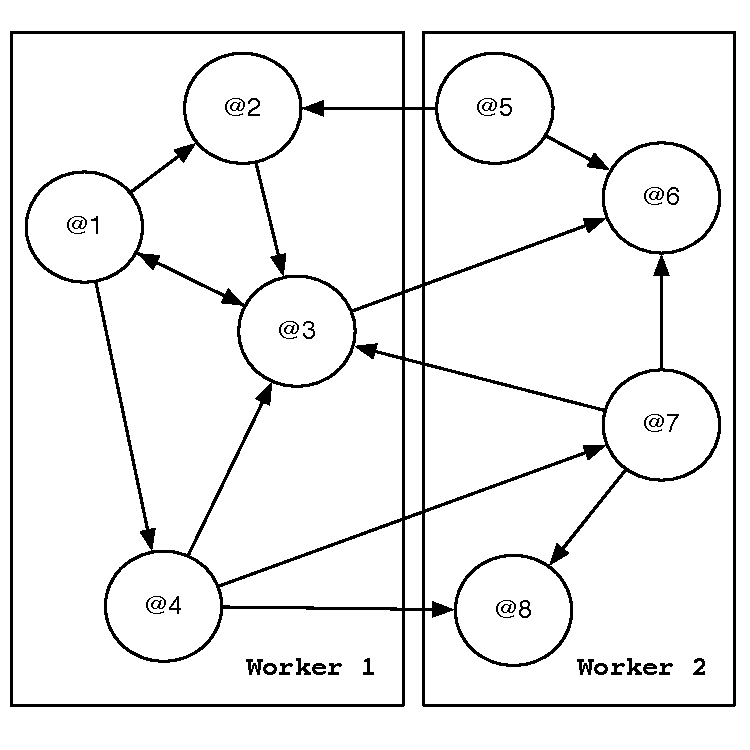
\includegraphics[height=5.5cm]{graph_coordination.pdf}
          \end{block}
          \column{.46\textwidth}
          \begin{block}{Coordination}
             {\small
             \begin{itemize}
                \item In LM we have $N$ nodes and $W$ workers/threads
                \item Graph of $N$ nodes is partitioned among the $W$ workers
             \end{itemize}
             }
          \end{block}
   \end{columns}
\end{frame}

\begin{frame}[fragile]
   \frametitle{Coordination}
   \begin{itemize}
      \item Due to linear facts, the order in which nodes are computed can affect either the final results and/or the speed of computation
      \begin{itemize}
         \item Randomized and approximation algorithms benefit from this because they can be computed faster
      \end{itemize}
      \item We use \emph{action facts} to tell the runtime system how to schedule computation
      \begin{itemize}
         \item Retracted once the runtime system makes the appropriate changes
      \end{itemize}
      \item \emph{Sensing facts} are used to sense the state of the runtime system
      \item We can write derivation rules that use sensing facts and then derive action facts
   \end{itemize}
\end{frame}

\begin{frame}[fragile]
   \frametitle{Coordination: Priorities}
   \begin{columns}[t]
         \column{.5\textwidth}
          \begin{block}{Example}
             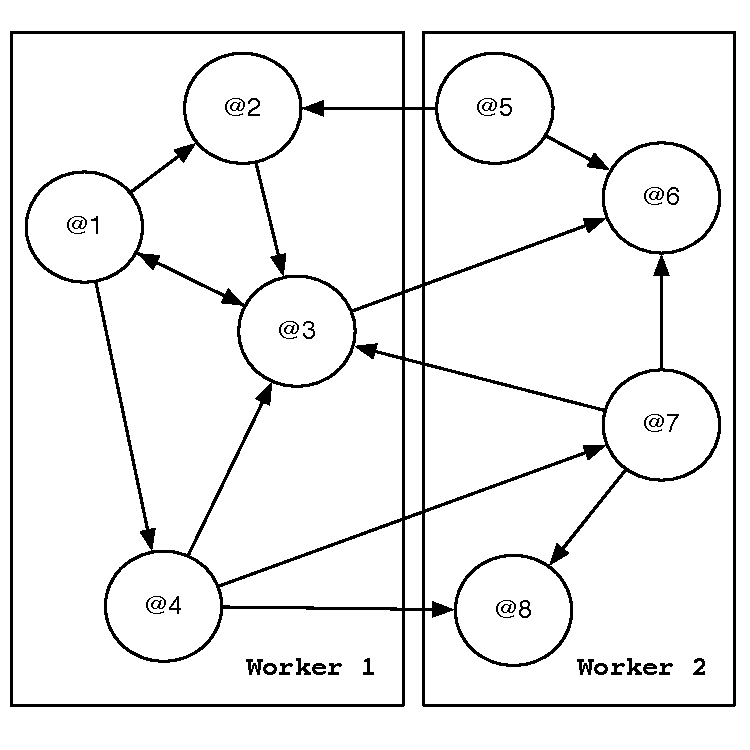
\includegraphics[height=5.5cm]{graph_coordination.pdf}
          \end{block}
          \column{.46\textwidth}
          \begin{block}{Coordination}
             {\small
             \begin{itemize}
                \item Programs are scheduled by changing the \emph{priority} of a node.
                \item High priority nodes are executed first
                \item Node priorities are taken into account at the worker level
             \end{itemize}
             }
          \end{block}
   \end{columns}
\end{frame}

\begin{frame}[fragile]
   \frametitle{Coordination Directives: Action Facts}
   \begin{itemize}
      \item \texttt{type linear action schedule-next(node)}: schedule node to run next.
      \item \texttt{type linear action set-priority(node, float)}: set the priority of a node. If the node already has some priority, we only change the priority if the new one is higher priority.
      \item \texttt{type linear action add-priority(node, float)}: get the current node's priority and increases or decreases it.
      \item \texttt{type linear action unset-priority(node)}: removes the priority, if any, from a given node.
      \item \texttt{type linear action stop-program(node)}: immediately stops the execution of the whole program.
   \end{itemize}
\end{frame}

\begin{frame}[fragile]
   \frametitle{Coordination Directives: Sensing Facts}
   \begin{itemize}
      \item \texttt{type linear cpu-id(node, node, int)}: the third argument indicates the worker's ID where the node of the second argument is currently running.
      \item \texttt{type linear priority(node, node, float)}: the third argument is the current priority of the node in the second argument.
   \end{itemize}
\end{frame}

\subsection{Shortest Distance}

\begin{frame}[fragile]
   \frametitle{Shortest Distance}
   \begin{columns}[t]
       \column{.5\textwidth}
       \begin{block}{Program}
         \begin{verbatim}[fontsize=\tiny,frame=single,commandchars=\\\{\}]
\alert[1]{type route edge(node, node, int).}
\alert[1]{type linear path(node, int, int).}

\alert[6]{priority @order asc.}

const visited = 1.
const notused = 0.

\alert[2]{path(startnode, 0, notused).}

\alert[3]{path(A, B, used),}
\alert[3]{path(A, B, notused)}
   \alert[3]{-o path(A, B, used).}

\alert[4]{path(A, B1, X),}
\alert[4]{path(A, B2, Y), B1 <= B2}
   \alert[4]{-o path(A, B1, X).}

\alert[5]{path(A, D, notused)}
   \alert[5]{-o \{B, W | !edge(A, B, W) |}
         \alert[5]{path(B, D + W, notused),}
         \alert[5,6]{set-priority(B, D + W))\},}
      \alert[5]{path(A, D, used).}
         \end{verbatim}
      \end{block}
      \column{.45\textwidth}
      \begin{block}{Explanation}
         {\small
         \begin{itemize}
            \only<1>{\item \texttt{edge/2} represents the edges between nodes
            \item \texttt{path/3} represents the distance to \texttt{startnode}
            \item The goal is to progressively compute the best \texttt{path/3} in all nodes}
            \only<2>{\item We start with distance 0 at \texttt{startnode}}
            
            \only<3>{\item First rule deletes unpropagated distance that was already propagated}
            \only<4>{\item Second rule deletes longer distances and keeps shorter distances}
            \only<5>{\item Third and final rule propagates distance to neighbor nodes}
            \only<6>{\item Node priorities are in ascending order (smaller is better)}
            \only<6>{\item When a distance is propagated, we set the target node priority to the new derived distance}
         \end{itemize}
         }
      \end{block}
   \end{columns}
\end{frame}

\subsection{Residual Splash BP}

\begin{frame}[fragile]
   \frametitle{Other coordinated programs}
   \begin{itemize}
      \item Heat Transfer
      \begin{itemize}
         \item Transfer heat values in a grid
         \item More heat transferred $\rightarrow$ higher priority
         \item Around $1.5$ times faster
      \end{itemize}
      \item $A^{*}$ Algorithm
      \begin{itemize}
         \item Search algorithm
         \item Priority of a node is dependent in how close the node is to the target
         \item 2 to 3 times better in a grid dataset
      \end{itemize}
      \item Residual Splash Belief Propagation~\cite{Gonzalez+al:aistats09paraml}
      \begin{itemize}
         \item Optimal strategy for parallelizing Loopy Belief Propagation~\cite{Murphy99loopybelief}
         \item Sum-Product message passing algorithm
      \end{itemize}
   \end{itemize}
\end{frame}

\begin{frame}[fragile]
   \frametitle{Residual Splash Belief Propagation}
   \begin{itemize}
      \item The strategy is to build a tree and then update the beliefs of each node twice, first from the leaves and then from the root
      \item The root of the tree is the node with the highest priority
      \begin{itemize}
         \item Highest priority $\rightarrow$ highest change in the delta of the belief value
         \item Priority is updated when the belief of a neighbor is computed
      \end{itemize}
      \item Each thread will build trees iteratively until the belief values converge
   \end{itemize}
   \begin{center}
      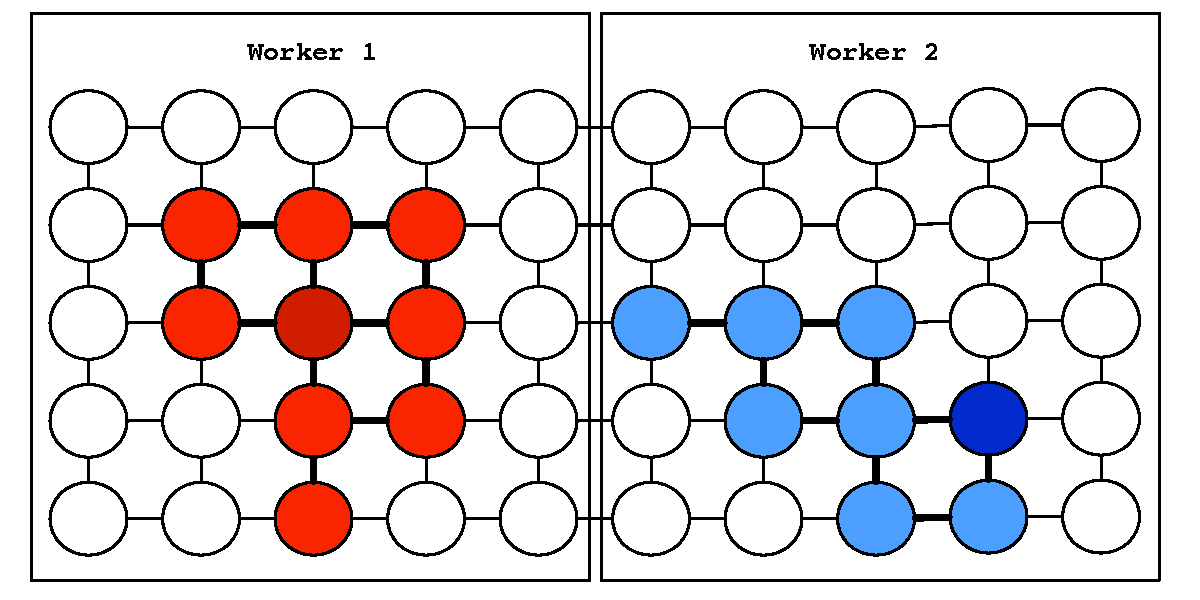
\includegraphics[height=5.1cm]{splash_bp.pdf}
   \end{center}
\end{frame}

\begin{frame}[fragile]
   \frametitle{Residual Splash Belief Propagation}
   \begin{block}{Tree Building}
   \begin{verbatim}[fontsize=\scriptsize,frame=single,commandchars=\\\{\}]
// end tree building
token(A, All, Next), length(All) > maxnodes
   -o first-phase(A, All, reverse(All)).
// expand tree
token(A, All, [A | Next])
   -o [collect => L | Side | !edge(A, L, Side),
         0 = count(All, L),
         0 = count(Next, L),
         \alert[1]{priority(A, L, P), P > 0.0},
         \alert[1]{cpu-id(A, L, Id1)},
         \alert[1]{cpu-id(A, A, Id2), Id1 = Id2} |
         send-token(A, All, Next ++ L)].

send-token(A, All, [])
   -o first-phase(A, All, reverse(All)).
send-token(A, All, [B | Next])
   -o \alert[1]{schedule-next(B)},
      token(B, All ++ [B], [B | Next]).
   \end{verbatim}
\end{block}
\end{frame}

\begin{frame}[fragile]
   \frametitle{Residual Splash Belief Propagation}
   \begin{block}{First Phase}
   \begin{verbatim}[fontsize=\scriptsize,frame=single,commandchars=\\\{\}]
first-phase(A, [A], [A]) -o second-phase(A, [], A).
first-phase(A, [A, B | Next], [A])
   -o update(A), \alert[1]{schedule-next(B)},
      second-phase(B, [B | Next], A).
first-phase(A, All, [A, B | Next])
   -o update(A), \alert[1]{schedule-next(B)},
      first-phase(B, All, [B | Next]).
   \end{verbatim}
\end{block}
   \begin{block}{Second Phase}
   \begin{verbatim}[fontsize=\scriptsize,frame=single,commandchars=\\\{\}]
second-phase(A, [], _)
   -o \alert[1]{unset-priority(A)}, waiting(A), update(A).
second-phase(A, [A], Back)
   -o update(A), waiting(Back),
      waiting(A), \alert[1]{unset-priority(A)}.
second-phase(A, [A, B | Next], Back)
   -o update(A), waiting(Back), \alert[1]{schedule-next(B)},
      second-phase(B, [B | Next], A).
   \end{verbatim}
\end{block}
\end{frame}

%
\section{Proof Theory}

\begin{frame}[fragile]
   \frametitle{Proof Theory}
   \begin{itemize}
      \item LM is based on a fragment of linear logic extended with definitions (for comprehensions and aggregates)
      \item Designed two dynamic semantics:
      \begin{itemize}
         \item High Level Dynamic (HLD) Semantics:
         \begin{itemize}
            \item Sequent calculus + focusing with positive atoms
            \item To apply a rule, \emph{focus} on the rule as an implication
            \item Rule selection and comprehension application are non-determinism and do not fully describe the behavior of LM
         \end{itemize}
         \item Low Level Dynamic (LLD) Semantics
         \begin{itemize}
            \item Close to the real implementation
            \item Describes rule selection and rule matching using a continuation stack
            \item Comprehensions are maximally applied
         \end{itemize}
      \end{itemize}
      \item The semantics model a single rule application:
      \begin{itemize}
         \item Input: Linear context ($\Delta$), Persistent Context ($\Gamma$), Rules ($\Phi$)
         \item Output: Derived Linear context ($\Delta'$), Derived Persistent context ($\Gamma'$), Consumed Linear context ($\Xi'$)
      \end{itemize}
   \end{itemize}
\end{frame}

\begin{frame}[fragile]
   \frametitle{Proof Theory: HLD}
   \begin{block}{Application}
\[
\infer[\az rule]
{\az \Gamma ; \Delta_1, \Delta_2 ; A \lolli B \rightarrow \Xi' ; \Delta' ; \Gamma'}
{\mz \Gamma ; \Delta_1 \rightarrow A & \dz \Gamma ; \Delta_2; \Delta_1; \cdot ; \cdot ; B \rightarrow \Xi' ; \Delta' ; \Gamma'}
\]

\[
\infer[\doz rule]
{\doz \Gamma ; \Delta ; R, \Phi \rightarrow \Xi' ; \Delta' ; \Gamma'}
{\az \Gamma ; \Delta ; R \rightarrow \Xi' ; \Delta' ; \Gamma'}
\]
   \end{block}
\end{frame}

\begin{frame}[fragile]
   \frametitle{Proof Theory: HLD}
   \begin{block}{Match}
\[
\infer[\mz 1]
{\mz \Gamma; \cdot \rightarrow 1}
{}
\tab
\infer[\mz p]
{\mz \Gamma; p \rightarrow p }
{}
\]

\[
\infer[\mz \bang p]
{\mz \Gamma, p; \cdot \rightarrow \bang p}
{}
\tab
\infer[\mz \otimes]
{\mz \Gamma; \Delta_1, \Delta_2 \rightarrow A \otimes B}
{\mz \Gamma; \Delta_1 \rightarrow A & \mz \Delta_2 \rightarrow B}
\]
   \end{block}
\end{frame}

\begin{frame}[fragile]
   \frametitle{Proof Theory: HLD}
   \begin{block}{Derivation}
{\small
      \[
\infer[\dz p]
{\dz \Gamma ; \Delta ; \Xi ; \Gamma_1 ; \Delta_1 ; p, \Omega \rightarrow \Xi' ; \Delta' ; \Gamma'}
{\dz \Gamma ; \Delta ; \Xi ; \Gamma_1 ; p, \Delta_1 ; \Omega \rightarrow \Xi' ; \Delta' ; \Gamma'}
\]

\[
\infer[\dz \bang p]
{\dz \Gamma ; \Delta ; \Xi ; \Gamma_1 ; \Delta_1 ; \bang p, \Omega \rightarrow \Xi' ; \Delta' ; \Gamma'}
{\dz \Gamma ; \Delta ; \Xi ; \Gamma_1, p ; \Delta_1 ; \Omega \rightarrow \Xi' ; \Delta' ; \Gamma'}
\]

\[
\infer[\dz \otimes]
{\dz \Gamma ; \Delta ; \Xi ; \Gamma_1 ; \Delta_1 ; A \otimes B, \Omega \rightarrow \Xi' ; \Delta' ; \Gamma'}
{\dz \Gamma ; \Delta ; \Xi ; \Gamma_1 ; \Delta_1 ; A, B, \Omega \rightarrow \Xi' ; \Delta' ; \Gamma'}
\]

\[
\infer[\dz 1]
{\dz \Gamma ; \Delta ; \Xi ; \Gamma_1; \Delta_1 ; 1, \Omega \rightarrow \Xi' ; \Delta' ; \Gamma'}
{\dz \Gamma ; \Delta ; \Xi ; \Gamma_1; \Delta_1 ; \Omega \rightarrow \Xi' ; \Delta' ; \Gamma'}
\]

\[
\infer[\dz end]
{\dz \Gamma ; \Delta ; \Xi' ; \Gamma' ; \Delta' ; \cdot \rightarrow \Xi' ; \Delta' ; \Gamma'}
{}
\]
}
   \end{block}
\end{frame}

\begin{frame}[fragile]
   \frametitle{Proof Theory: HLD}
   \begin{block}{Derivation}
{\small
      \[
      \infer[\dz comp]
      {\dz \Gamma ; \Delta ; \Xi ; \Gamma_1 ; \Delta_1 ; \comp A \lolli B, \Omega \rightarrow \Xi' ; \Delta' ; \Gamma'}
      {\dz \Gamma ; \Delta ; \Xi ; \Gamma_1 ; \Delta_1 ; 1 \with (A \lolli B \otimes \comp A \lolli B), \Omega \rightarrow \Xi' ; \Delta' ; \Gamma'}
      \]

      \[
      \infer[\dz \lolli]
      {\dz \Gamma ; \Delta_a, \Delta_b ; \Xi ; \Gamma_1 ; \Delta_1 ; A \lolli B, \Omega \rightarrow \Xi' ; \Delta' ; \Gamma'}
      {\mz \Gamma ; \Delta_a \rightarrow A & \dz \Gamma ; \Delta_b ; \Xi, \Delta_a ; \Gamma_1 ; \Delta_1 ; B, \Omega \rightarrow \Xi' ; \Delta' ; \Gamma'}
      \]

      \[
      \infer[\dz \with L]
      {\dz \Gamma ; \Delta ; \Xi ; \Gamma_1 ; \Delta_1 ; A \with B, \Omega \rightarrow \Xi' ; \Delta'; \Gamma'}
      {\dz \Gamma ; \Delta ; \Xi ; \Gamma_1 ; \Delta_1 ; A, \Omega \rightarrow \Xi' ; \Delta'; \Gamma'}
      \]

      \[
      \infer[\dz \with R]
      {\dz \Gamma ; \Delta ; \Xi ; \Gamma_1 ; \Delta_1 ; A \with B, \Omega \rightarrow \Xi' ; \Delta' ; \Gamma'}
      {\dz \Gamma ; \Delta ; \Xi ; \Gamma_1 ; \Delta_1 ; B, \Omega \rightarrow \Xi' ; \Delta' ; \Gamma'}
      \]
      }
   \end{block}
\end{frame}

\begin{frame}[fragile]
   \frametitle{Proof Theory: LLD}
   \begin{block}{LLD Semantics Example}
      \includegraphics<1>[height=6.5cm]{lld1.pdf}
      \includegraphics<2>[height=6.5cm]{lld2.pdf}
      \includegraphics<3>[height=6.5cm]{lld3.pdf}
      \includegraphics<4>[height=6.5cm]{lld4.pdf}
      \includegraphics<5>[height=6.5cm]{lld5.pdf}
      \includegraphics<6>[height=6.5cm]{lld6.pdf}
      \includegraphics<7>[height=6.5cm]{lld7.pdf}
      \includegraphics<8>[height=6.5cm]{lld8.pdf}
      \includegraphics<9>[height=6.5cm]{lld9.pdf}
      \includegraphics<10>[height=6.5cm]{lld10.pdf}
   \end{block}
\end{frame}

\begin{frame}[fragile]
   \frametitle{Proof Theory: Soundness Proof}
   \begin{itemize}
      \item Every proof/execution performed in LLD can also be done in HLD (soundness)
      \item Contents of each continuation frame are important:
      \begin{itemize}
         \item Remaining terms to match
         \item Previous matched terms
         \item Available facts and consumed facts
         \item Remaining facts to try
      \end{itemize}
      \pause
      \item Critical points of the proof:
      \begin{itemize}
         \item Maintaining the well-formedness of the continuation stack at all times
         \item Stack must be related to a term $A$ (term to prove) and to the initial database
         \item Comprehensions and databases work by re-using the stack as many times as many backtracks are possible (database iteration!)
      \end{itemize}
      \pause
      \item On the other hand, completeness cannot be proven!
      \pause
      \item Connection between the dynamic semantics of LM and linear logic is established
      \begin{itemize}
         \item Implementation is close enough to LLD semantics
      \end{itemize}
   \end{itemize}
\end{frame}

\section{Current Implementation}

\begin{frame}[fragile]
   \frametitle{Implementation}
   \begin{itemize}
      \item Virtual Machine + Compiler
      \item Compiler compiles code into byte-code
      \item Virtual machine is written in C++ and uses pthreads to parallelize execution
      \item Preliminary distributed implementation using MPI and a blinky blocks implementation
      \item Graph is initially partitioned among the $T$ threads
      \begin{itemize}
         \item Nodes are ordered by the compiler for improved data locality
         \item For load balancing, node stealing is employed whenever a thread is about to become idle
      \end{itemize}
   \end{itemize}
\end{frame}

\begin{frame}[fragile]
   \frametitle{Compiler}
   \begin{itemize}
      \item We compile each rule into a list of instructions and a list of predicates needed to match the rule
      \item Rule \texttt{!a(X,Y), b(X,Z), c(X,Y) -o d(Y)}:
      \begin{block}{Byte-Code}
         \scriptsize\begin{verbatim}
PERSISTENT ITERATE a MATCHING TO reg 0
  LINEAR ITERATE b MATCHING TO reg 1
      (match).0=0.0
    LINEAR ITERATE c MATCHING TO reg 2
        (match).0=0.0
        (match).1=0.1
      ALLOC d TO reg 3
      MVFIELDFIELD 0.1 TO 3.0
      ADDLINEAR reg 3
      REMOVE reg 2
      REMOVE reg 1
      TRY NEXT
    NEXT
  NEXT
RETURN
         \end{verbatim}
      \end{block}
   \end{itemize}
\end{frame}

\begin{frame}[fragile]
   \frametitle{Virtual Machine}
   \begin{itemize}
      \item Active nodes have unprocessed facts and pending rules to execute
      \item Data structures to store facts:
      \begin{itemize}
         \item Tries: for persistent facts
         \item Doubly linked lists: for linear facts (easy to remove and add)
         \item Hash table: for indexing linear facts (indexed by one argument)
      \end{itemize}
      \item Threads synchronize when they execute a node and need to send a fact to a node in another thread
      \begin{itemize}
         \item Thread needs to lock internal node data structures in order to manage the rule engine
         \item Each node maintains an efficient data structure to decide which rules, given priorities, need to be executed 
      \end{itemize}
   \end{itemize}
\end{frame}

\begin{frame}[fragile]
   \frametitle{Virtual Machine}
   \begin{itemize}
      %\item A global counter and an active/inactive flag for each thread is used to detect termination
      \item Each thread has two queues:
      \begin{itemize}
         \item Normal queue: doubly linked list of active nodes
         \item Priority queue: heap data structure of active nodes
         \item Active nodes are either in the normal queue or priority queue
         \item Both queues are protected by locks
      \end{itemize}
      \item Coordination directives are implemented as VM instructions
      \item Right now, only coordination directives that execute on the nodes of the same thread are taken into account
   \end{itemize}
\end{frame}

\begin{frame}[fragile]
   \frametitle{Virtual Machine}
   \begin{block}{Work Loop}
   \scriptsize
\begin{verbatim}
void work_loop(thread_id tid):
   while (true):
      current_node = NULL;
      if(has_work(tid)):
         current_node = priority_queue.pop_work(tid)
         if current_node == NULL:
            current_node = normal_queue.pop_work(tid);
      else:
         target_thread = random(NUM_THREADS);
         // need to steal a node
         for (i = 0; i < NUM_THREADS && current_node == NULL; ++i):
            target_thread = (target_thread + 1) % NUM_THREADS;
            current_node = steal_node_from_thread(target_thread)
      if(current_node == NULL):
         become_idle(tid);
         if(!synchronize_termination(tid)):
            return;
         become_active(tid);
      else:
         process_node(current_node, tid);
   \end{verbatim}
   \end{block}
\end{frame}

\section{Experimental Results}

\begin{frame}[fragile]
   \frametitle{Experimental Results: Scalability}
   \begin{columns}[t]
      \column{.5\textwidth}
      \begin{figure}[b]
         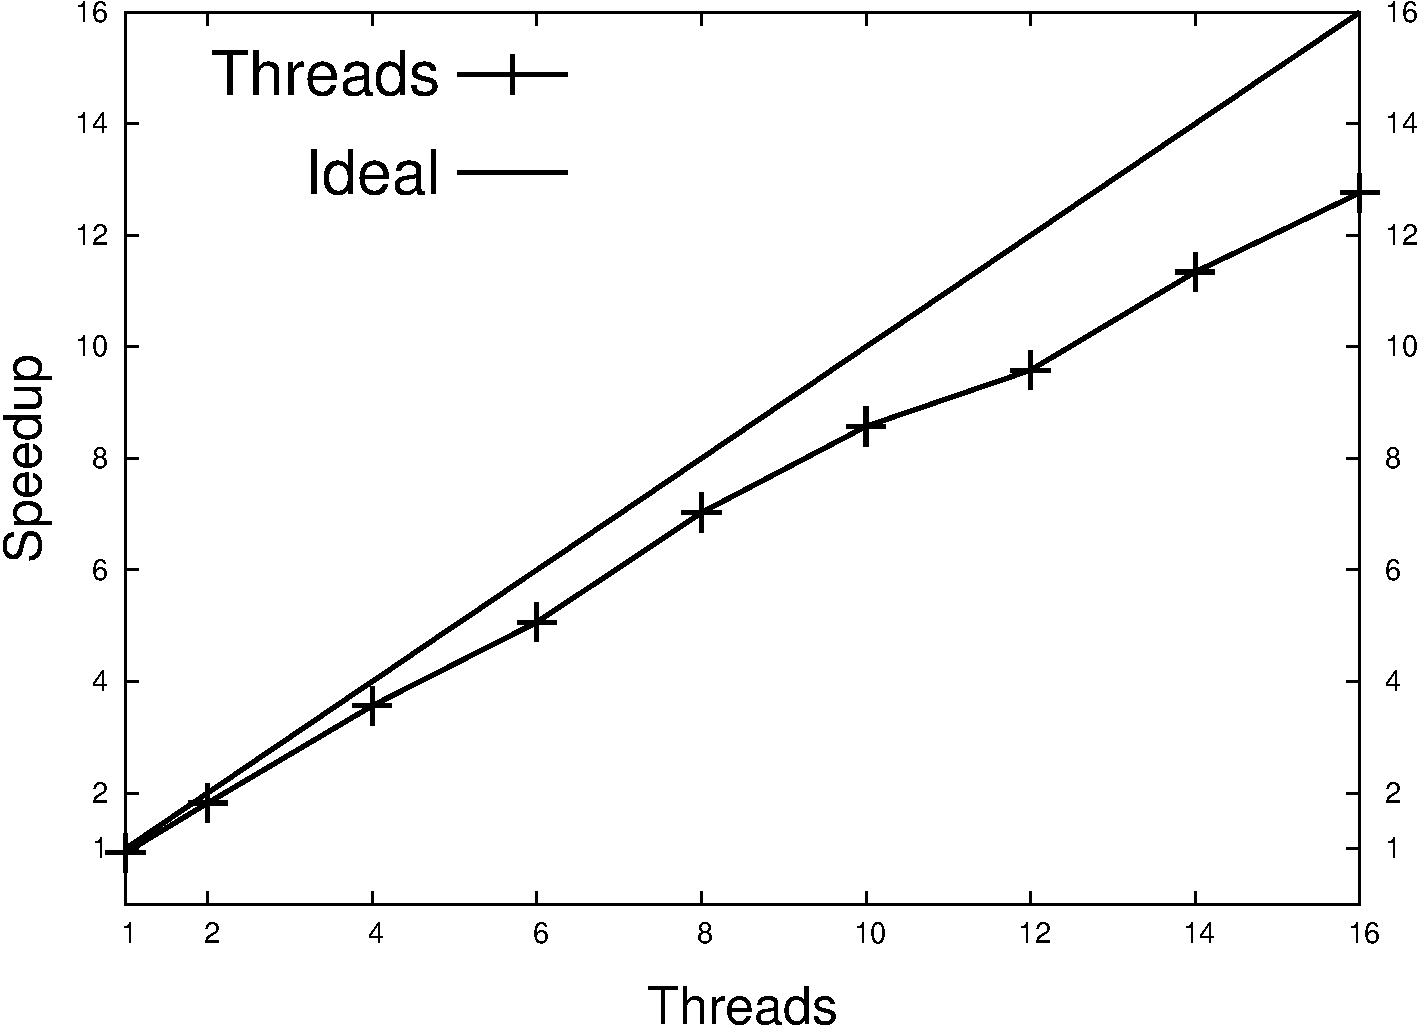
\includegraphics[width=\textwidth]{speedup_8queens-13.pdf}
         \caption{N-Queens program (13x13~board)}
      \end{figure}
      \column{.5\textwidth}
      \begin{figure}[b]
         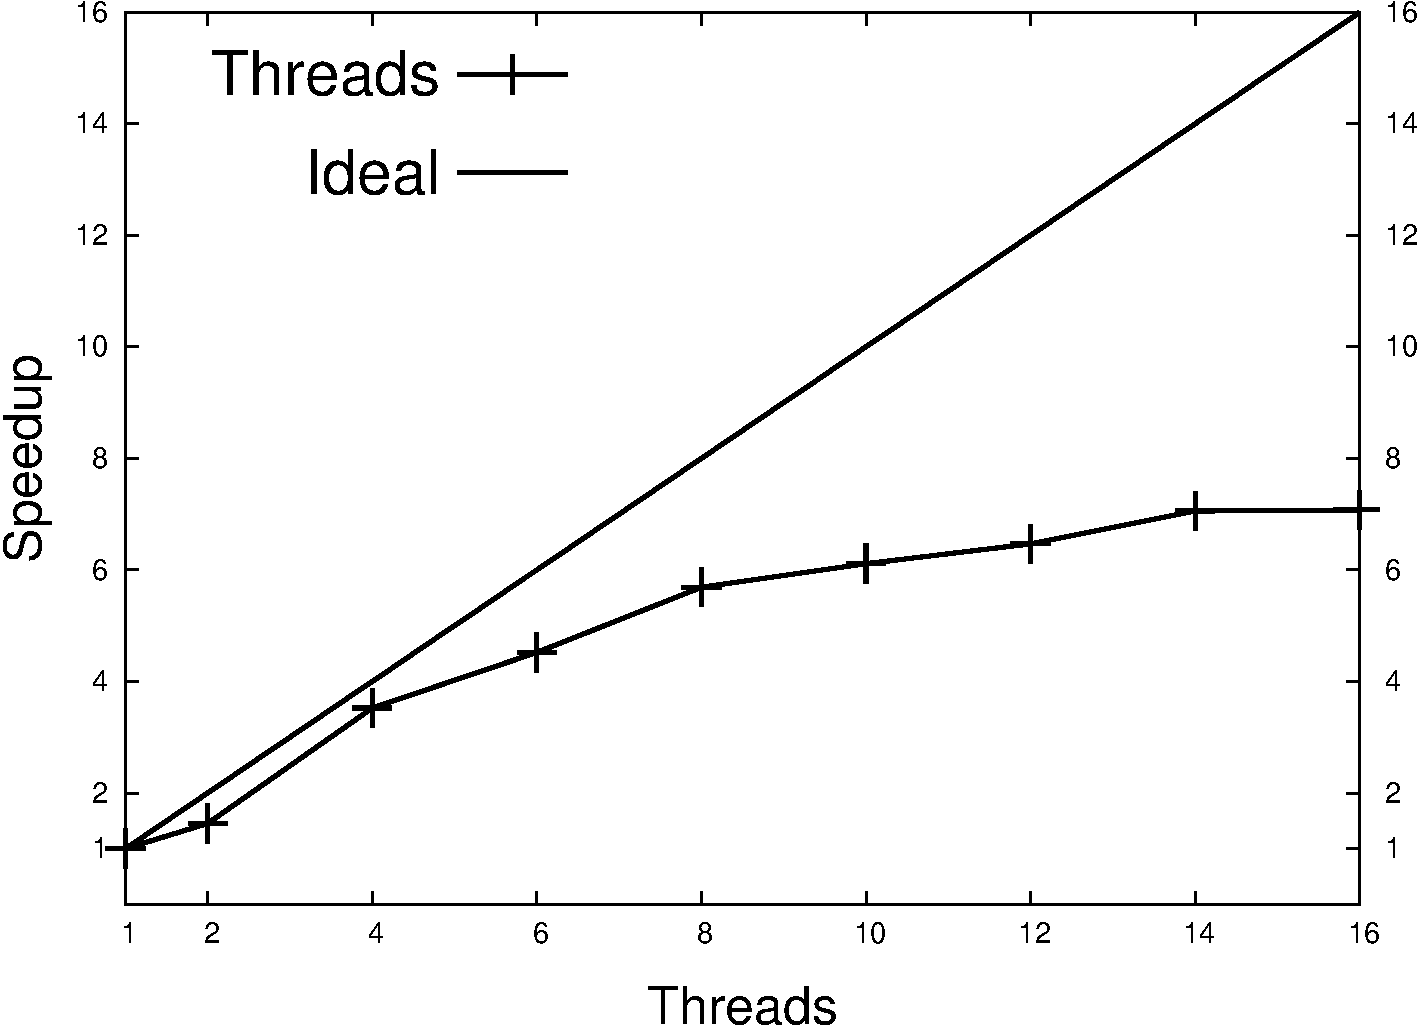
\includegraphics[width=\textwidth]{speedup_greedy-graph-coloring-search_engines.pdf}
         \caption{Greedy Graph Coloring: using a graph of web pages.}
      \end{figure}
   \end{columns}
\end{frame}

\begin{frame}[fragile]
   \frametitle{Experimental Results: Scalability}
   \begin{figure}[b]
      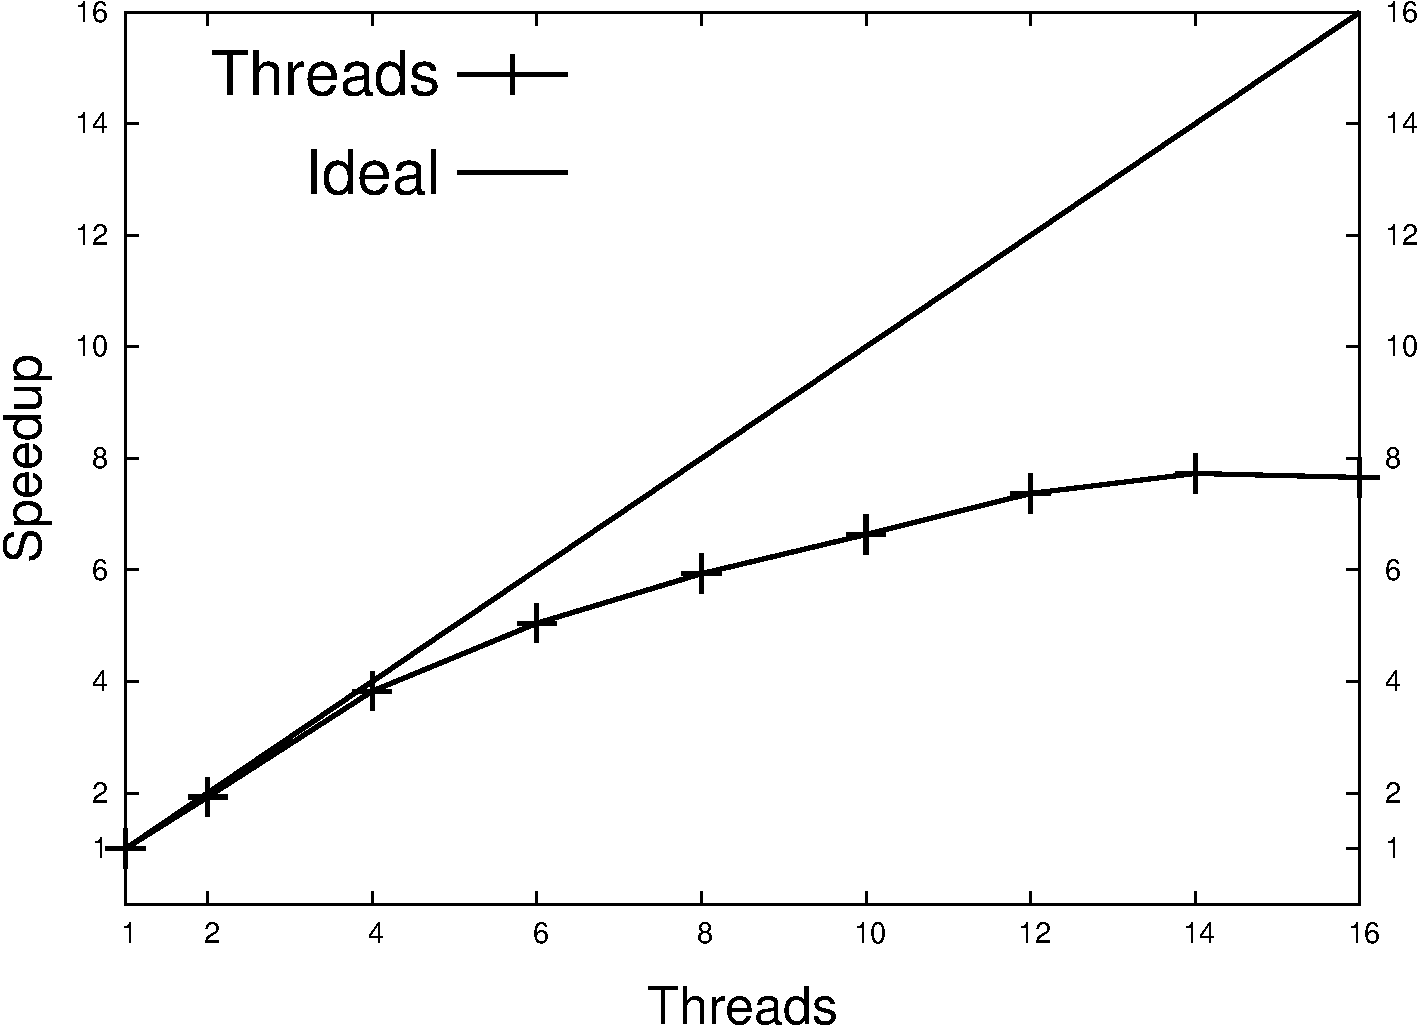
\includegraphics[width=0.5\textwidth]{speedup_pagerank-search_engines.pdf}
      \caption{Asynchronous PageRank: using a graph of web pages.}
   \end{figure}
\end{frame}

\begin{frame}[fragile]
   \frametitle{Experimental Results: Coordination}
   \begin{columns}[t]
      \column{.5\textwidth}
      \begin{figure}[b]
         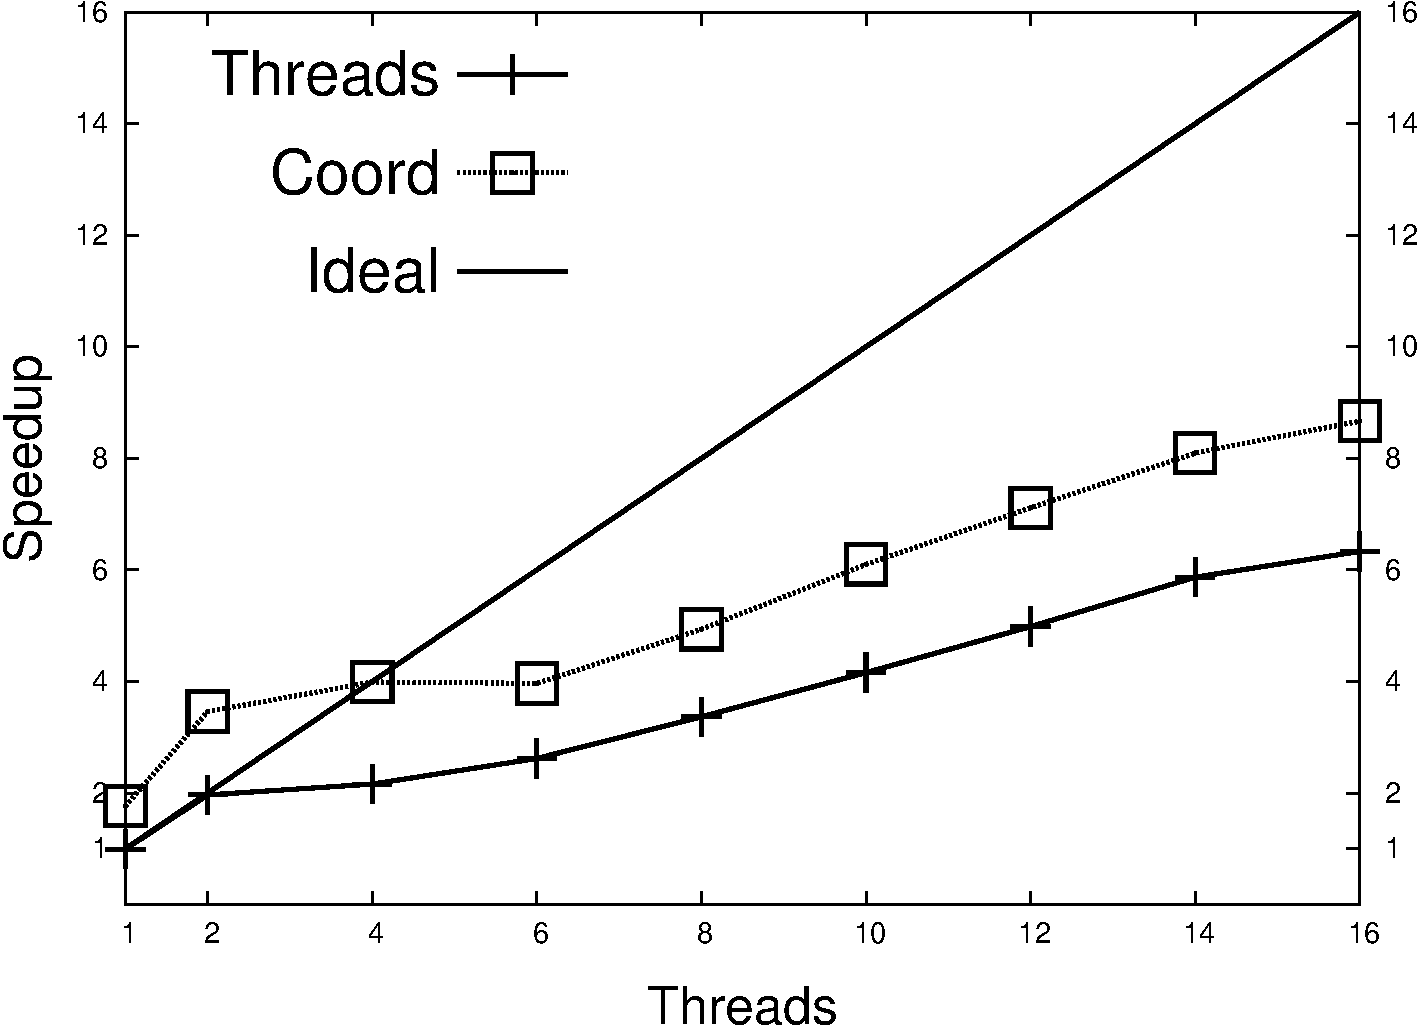
\includegraphics[width=\textwidth]{coord/speedup_heat-transfer-80.pdf}
         \caption{Heat transfer program: using a grid dataset}
      \end{figure}
      \column{.5\textwidth}
      \begin{figure}[b]
         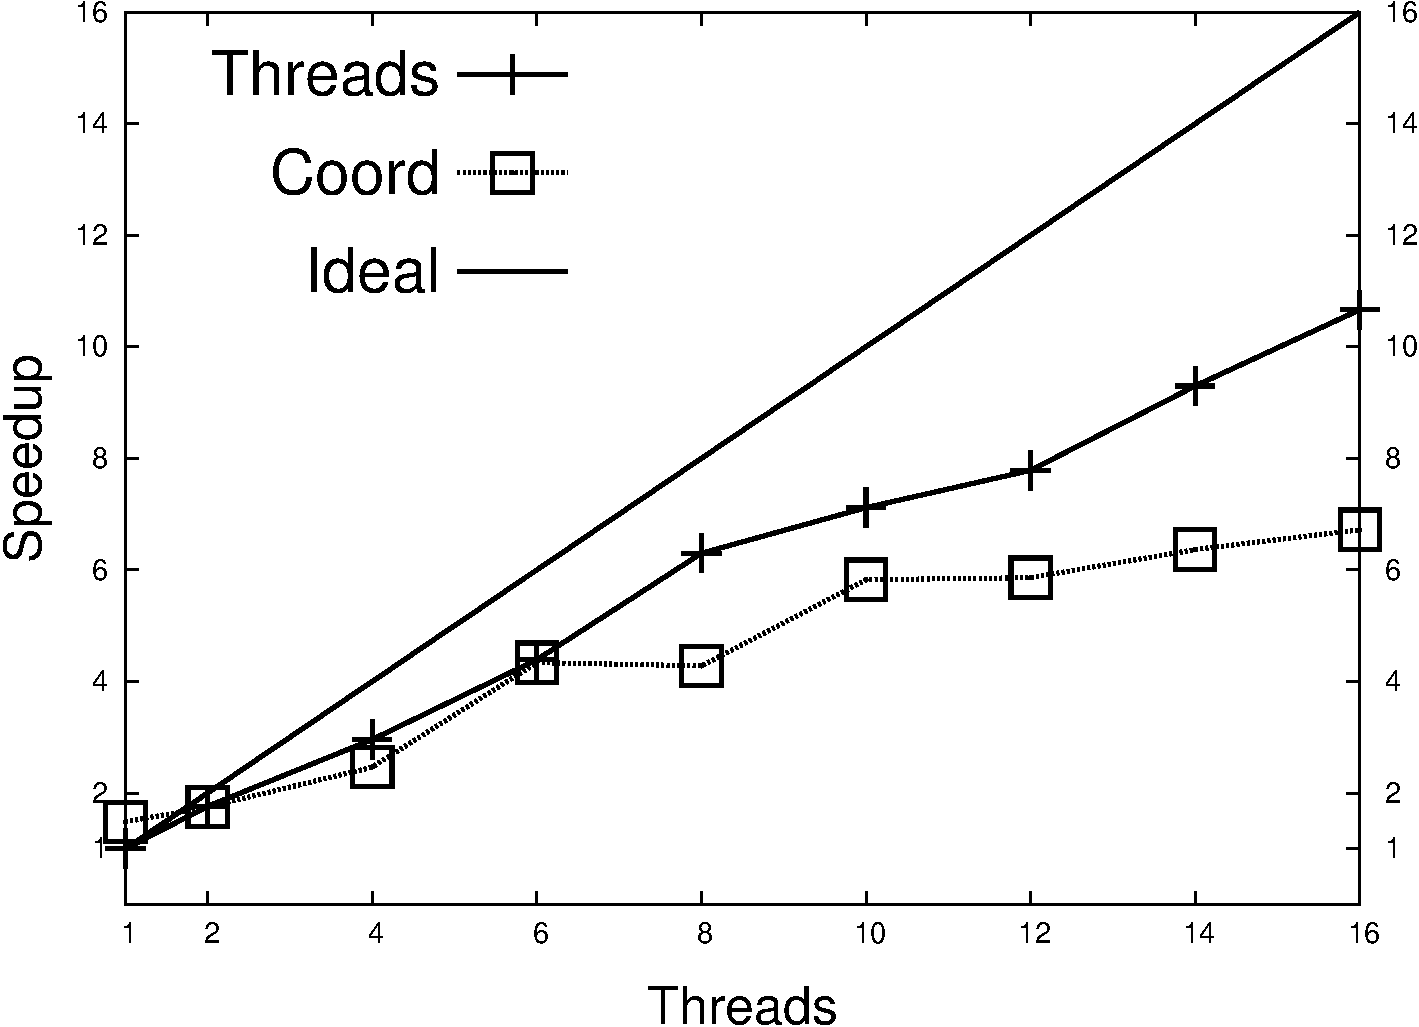
\includegraphics[width=\textwidth]{coord/speedup_shortest-uspowergrid.pdf}
         \caption{Shortest Distance: using US Power Grid dataset}
      \end{figure}
   \end{columns}
\end{frame}

\begin{frame}[fragile]
   \frametitle{Experimental Results: Coordination}
   \begin{columns}[t]
      \column{.5\textwidth}
      \begin{figure}[b]
         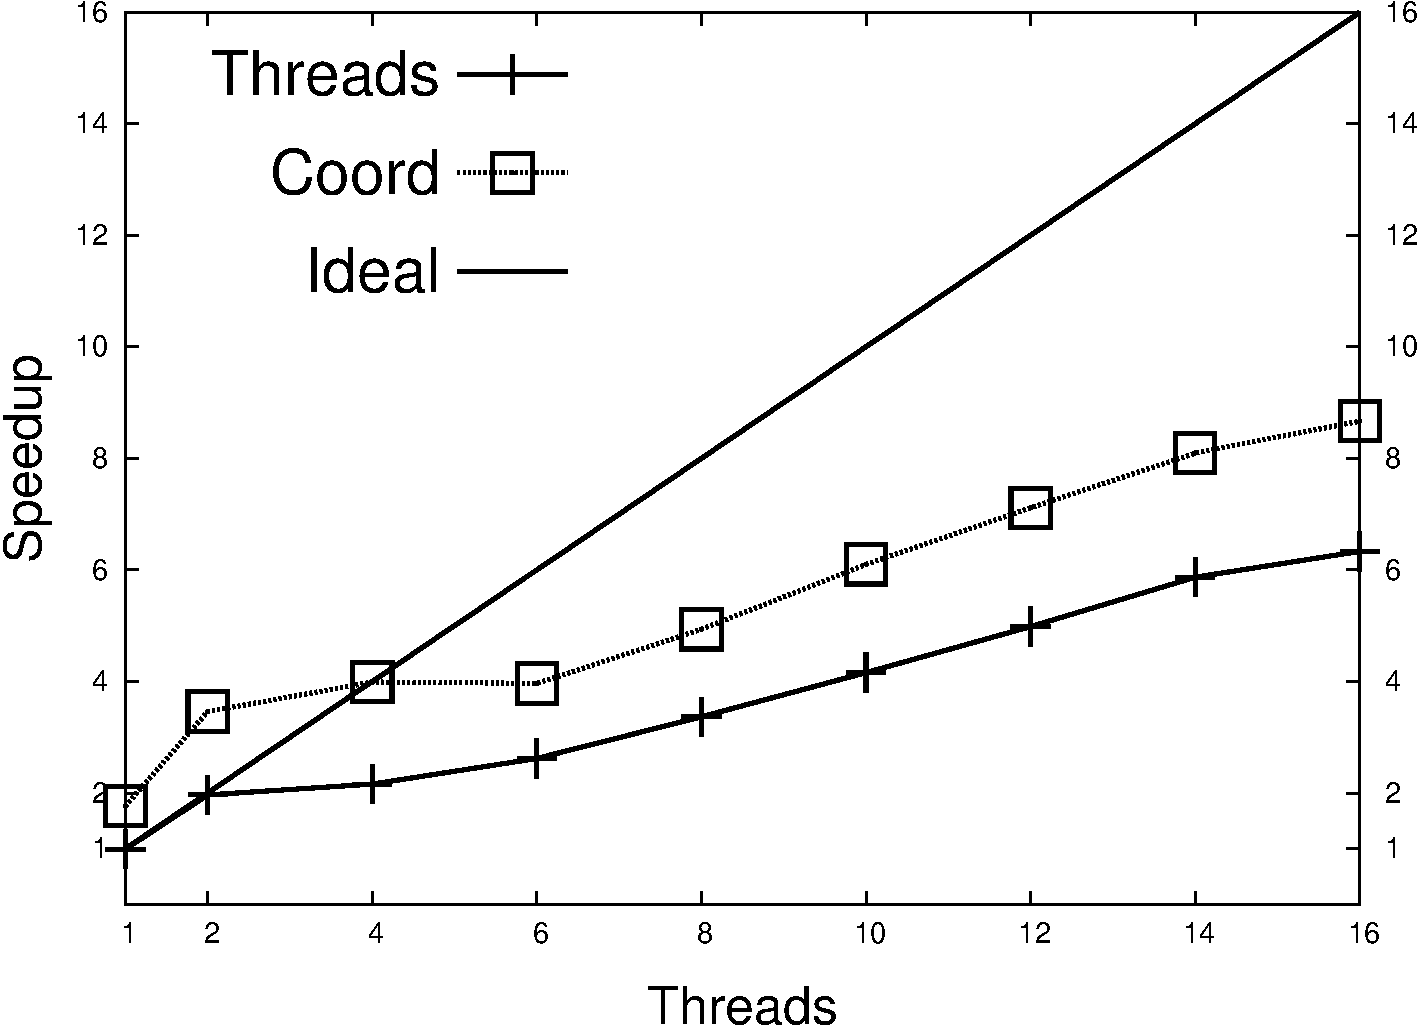
\includegraphics[width=\textwidth]{coord/speedup_heat-transfer-80.pdf}
         \caption{Heat transfer program: using a grid dataset}
      \end{figure}
      \column{.5\textwidth}
      \begin{figure}[b]
         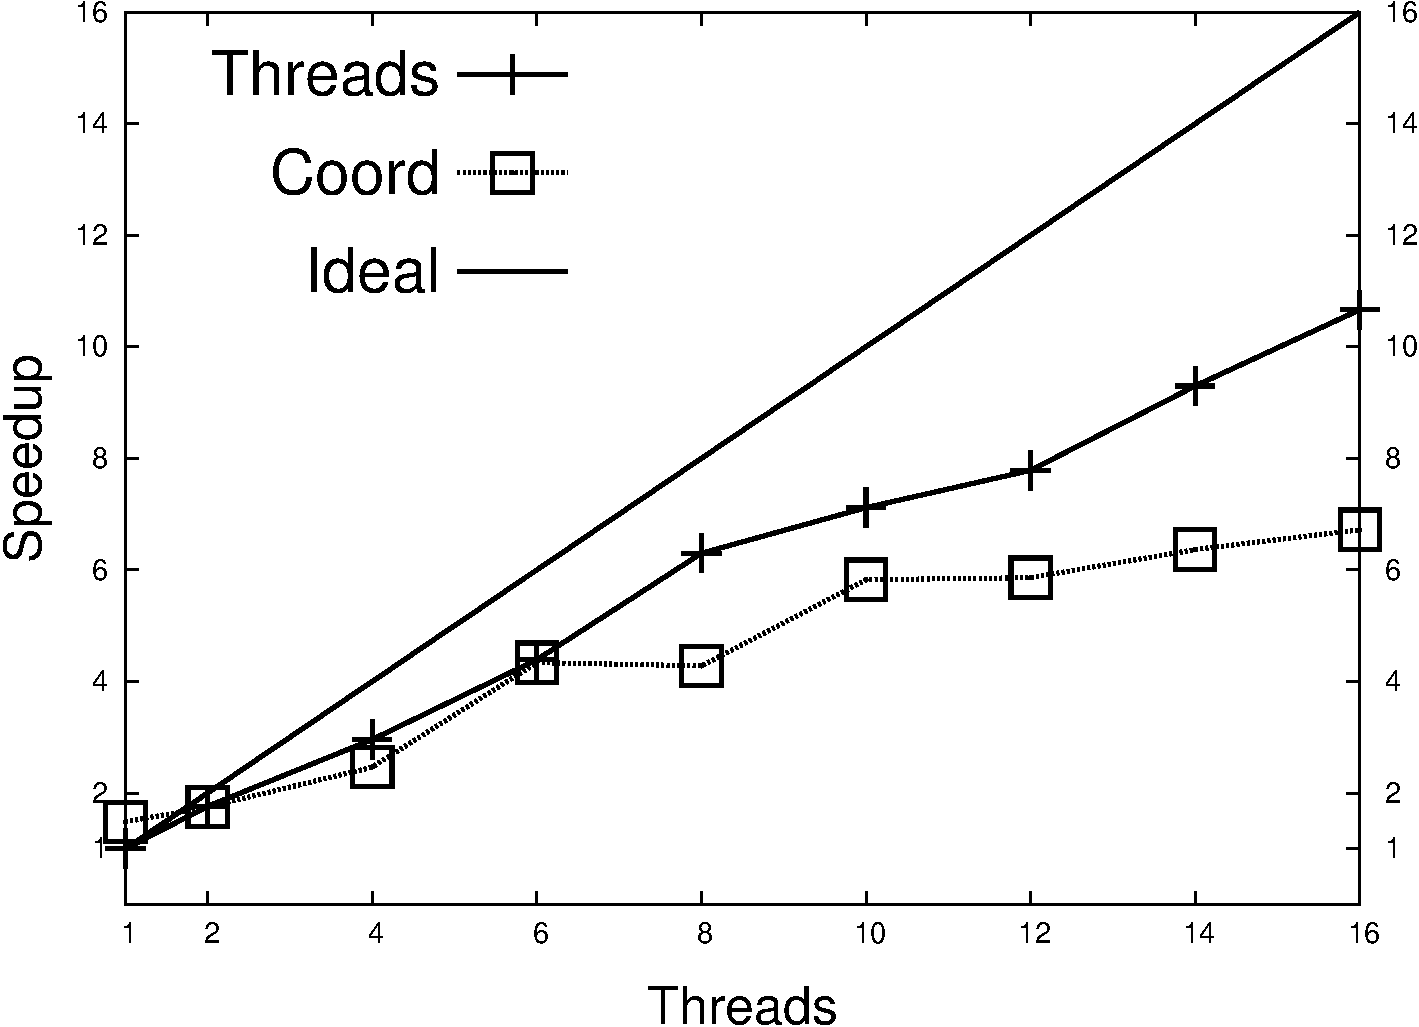
\includegraphics[width=\textwidth]{coord/speedup_shortest-uspowergrid.pdf}
         \caption{Shortest Distance: using US Power Grid dataset}
      \end{figure}
   \end{columns}
\end{frame}

\begin{frame}[fragile]
   \frametitle{Experimental Results: Coordination}
   \begin{columns}
      \column{.3\textwidth}
      \begin{figure}[b]
         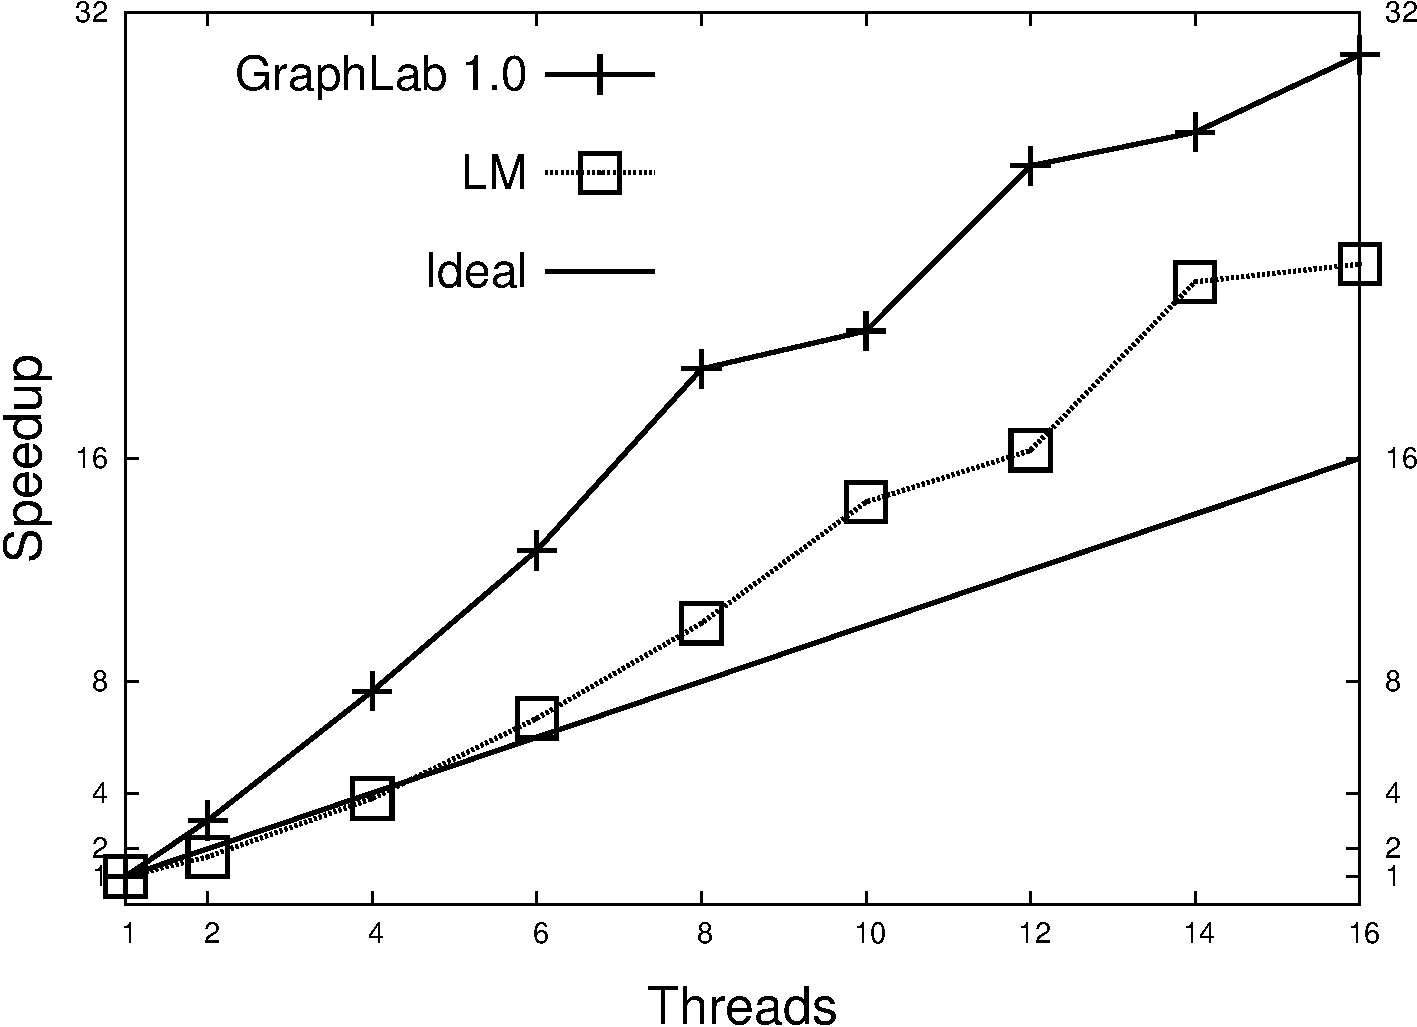
\includegraphics[width=\textwidth]{coord/speedup_bp-graphlab-400.pdf}
         \caption{Basic BP without splashes\newline\newline}
      \end{figure}
      \column{.3\textwidth}
      \begin{figure}[b]
         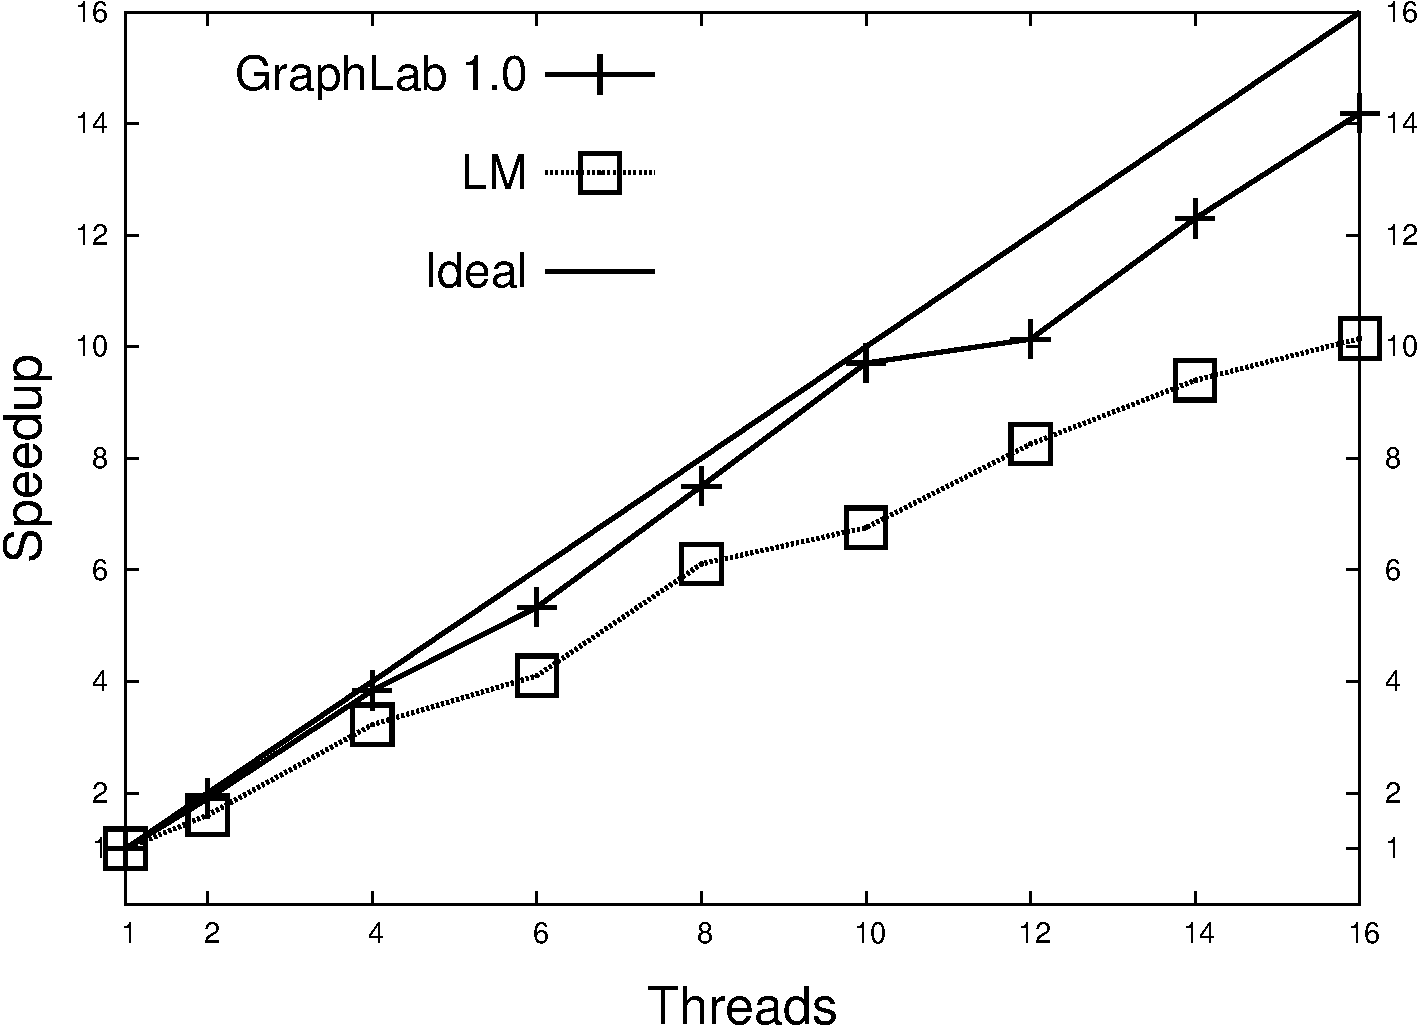
\includegraphics[width=\textwidth]{coord/speedup2_bp-graphlab-400.pdf}
         \caption{BP with splashes\newline\newline}
      \end{figure}
      \column{.3\textwidth}
      \begin{figure}[b]
         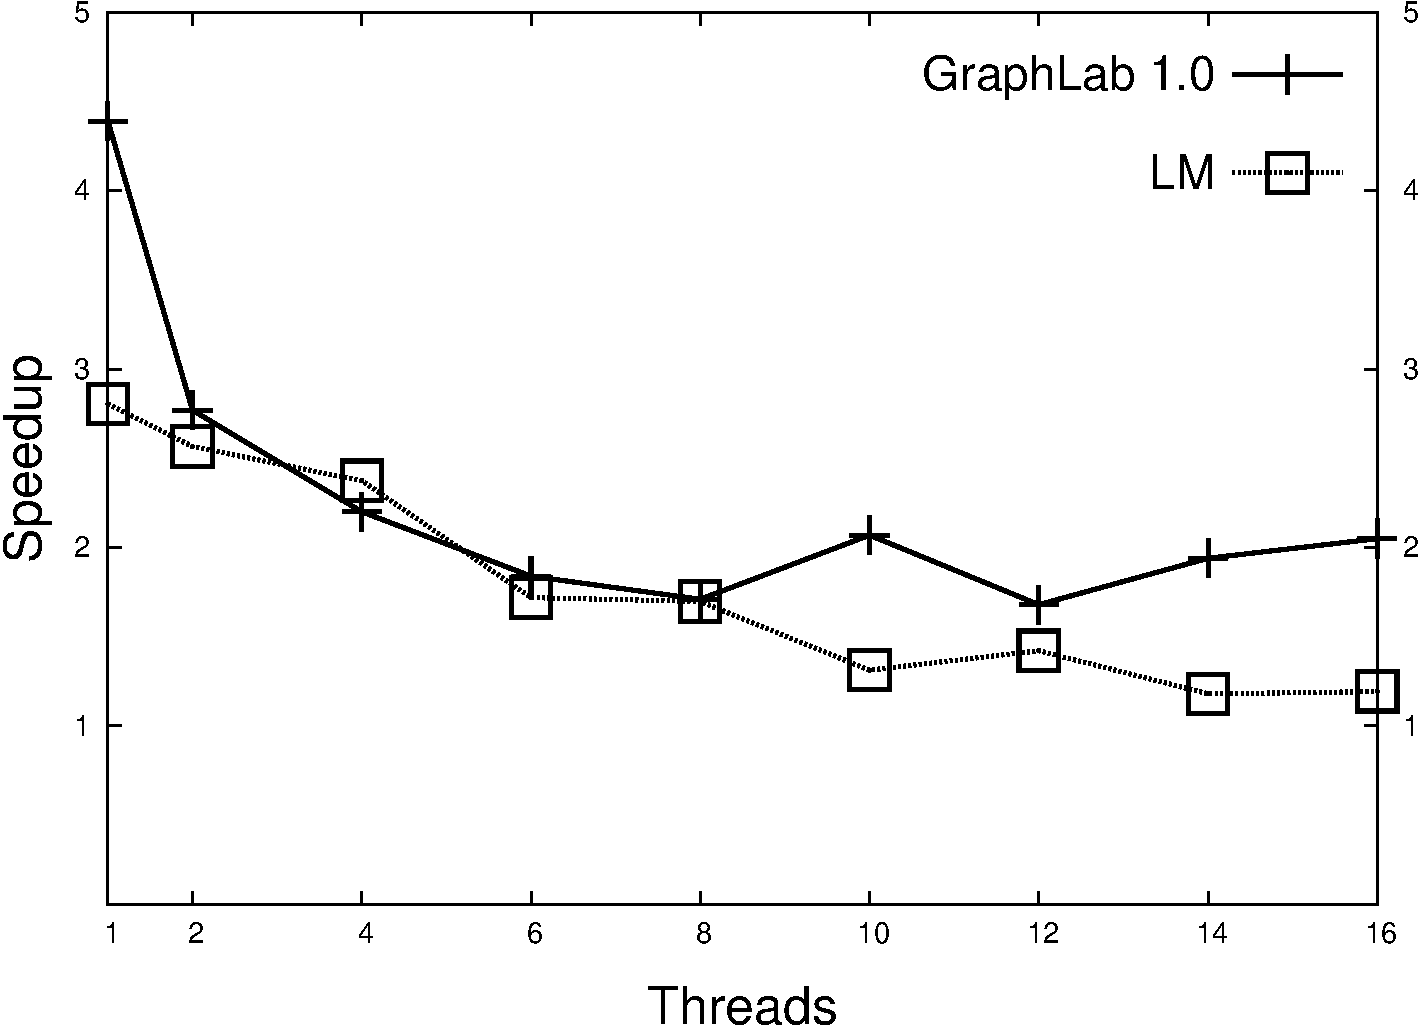
\includegraphics[width=\textwidth]{coord/improv_bp-graphlab-400.pdf}
         \caption{Coordination improvements of BP with splashes over basic BP}
      \end{figure}
   \end{columns}
\end{frame}

\begin{frame}[fragile]
   \frametitle{Experimental Results: Absolute Execution Time}
   \begin{figure}[b]
      \begin{tabular}{ | l | l | l | l |}
       \hline

       Size & C & Python & YAP Prolog \\ \hline\hline
       10 & 16.92 & \textbf{0,62} & 5,42 \\
       11 & 21.59 & \textbf{0.64} & 6.47 \\
       12 & 10.32 & \textbf{0.73} & 7.61 \\
       13 & 14.35 & \textbf{0.88} & 10.38 \\
       \hline
       \end{tabular}
       \caption{N-Queens problem.}
    \end{figure}
    \begin{figure}[b]
       \begin{tabular}{ | l | l | l | l |}
        \hline

        Size & C & Python & GraphLab \\ \hline\hline
        10 & \textbf{0.67} & \textbf{0,03} & \textbf{1.00} \\
        50 & \textit{1.77} & \textbf{0.04} & \textit{1.73} \\
        200 & \textit{1.99} & \textbf{0.05} & \textit{1.79} \\
        400 & \textit{2.00} & \textbf{0.04} & \textit{1.80} \\
        \hline
        \end{tabular}
        \caption{Belief Propagation program.}
    \end{figure}
\end{frame}

\begin{frame}[fragile]
   \frametitle{Language Expressiveness and Conciseness}
   \begin{table}[ht]
   \begin{center}
      \resizebox{12cm}{!}{
       \begin{tabular}{| c | c | l | c |}
       \hline
       \textbf{Program} & \textbf{LM} & \textbf{Others} & \textbf{Average} \\ \hline \hline
       SSSP & 6 & 25 (C++) & 24\% \\ \hline
       PageRank & 30 & 60 (GraphLab) & 50\% \\ \hline
       BP & 50 & 90 (GraphLab) & 55\% \\ \hline
       Splash BP & 50 & 350 (GraphLab) & 14\% \\ \hline
       N Queens & 40 & 300 (C~\cite{8queens-parallel}), 400 (MPI~\cite{Rolfe:2008:SMA:1473195.1473217}) & 11\% \\ \hline
       \end{tabular}}
   \end{center}
        \caption{Comparison of source code size against other languages.}
   \end{table}
\end{frame}

\section{Roadmap}

\begin{frame}[fragile]
   \frametitle{First Goal: Improved Coordination Mechanism}
   \begin{itemize}
      \item Coordination directives show potential in improving execution of programs, although our system shows some problems when using it with several threads
      \begin{itemize}
         \item We need an efficient design for sharing coordination information between threads
         \item Coordination time + Execution time $<$ Uncoordinated execution time
      \end{itemize}
      \item We also need more programs that use coordination in order to design more useful coordination directives
      \begin{itemize}
         \item Programs where data locality matters: may be more important in distributed systems
         \item Decision tree algorithms?
         \item Neural network pruning? (improved back propagation during training)
         \item Alpha-Beta algorithm?
      \end{itemize}
      \item Due to new multicore architectures and traditional distributed systems it might be useful to also see the processing units as a graph
      \begin{itemize}
         \item Useful for data locality
         \item Improved use of the L2 cache?
         \item New sensing facts
      \end{itemize}
   \end{itemize}
\end{frame}

\begin{frame}[fragile]
   \frametitle{Second Goal: Improved parallelism}
   \begin{itemize}
      \item In our results, there are some scalability problems as the number of threads increases to 32 and 64
      \item There's still some room for improvement in terms of thread management:
      \begin{itemize}
         \item Improve node stealing algorithm
      \end{itemize}
      \item Measure and instrument the virtual machine to better understand how threads behave during execution
   \end{itemize}
\end{frame}

\begin{frame}[fragile]
   \frametitle{Third Goal: Compilation and Runtime Improvements}
   \begin{itemize}
      \item Improve absolute running time of LM programs and make LM more competitive
      \item It is possible to take advantage of the fact that LM is a logic programming language in order to simplify and optimize programs
      \item Compiler should detect code invariants such as:
      \begin{itemize}
         \item Property linear facts: each node has a single fact of a predicate that is consumed but re-derived immediately with updated arguments
         \item Triggering linear facts: some facts never trigger new rules (example: they are property facts)
         \item Single use facts: linear facts that once derived are known to immediately derive a rule
      \end{itemize}
      \item Measure the impact of such optimizations
   \end{itemize}
\end{frame}

\begin{frame}[fragile]
   \frametitle{Optional Goal: Program correctness}
   \begin{itemize}
      \item Some work has already been done to prove properties of linear logic programs.
      \item Robert Simmons employed an approach called generative invariants~\cite{simmons:Thesis} to prove that an operational semantics of a programming language follows some invariants, namely type preservation
      \item It may be possible to prove invariants about our programs, including correctness and termination invariants
   \end{itemize}
\end{frame}

\begin{frame}[fragile]
   \frametitle{Timeline}
   \begin{itemize}
      \item Fall 2014
      \begin{itemize}
         \item Measure sources of overhead of the VM and apply required optimizations
         \item Improve scalability of current coordination mechanisms
         \item Write 1 or 2 new coordinated programs and extend the set of coordination directives if needed
      \end{itemize}
      \item Spring 2014
      \begin{itemize}
         \item Design a set of invariant optimizations and implement them
         \item Benchmark programs to see how they are improved
         \item Write 1 or 2 new coordinated programs
         \item Continue working on scalability optimizations
      \end{itemize}
      \item Summer 2015
      \begin{itemize}
         \item Finish the previous tasks
         \item Write the thesis document
      \end{itemize}
   \end{itemize}
\end{frame}

\begin{frame}[fragile]
   \frametitle{Publications}
   \begin{thebibliography}{9}
      \bibitem{damp} Bottom-up logic programming for multicores. In Proceedings of the Workshop on Declarative Aspects of Multicore Programming, DAMP'12, Philadelphia, PA, January 2012. ACM Press
      \bibitem{iclp}A Linear Logic Programming Language for Concurrent Programming over Graph Structures. Journal of Theory and Practice of Logic Programming, 30th International Conference on Logic Programming (ICLP 2014), Special Issue, Cambridge University Press
      \bibitem{logcom} Dynamic Semantics for a Concurrent Forward-Chaining Linear Logic Programming Language (In preparation)
      \bibitem{ciclops} A Parallel Virtual Machine for Executing Forward-Chaining Linear Logic Programs. 14th Colloquium on Implementation of Constraint and LOgic Programming Systems (CICLOPS 2014)
   \end{thebibliography}
   
\end{frame}

\begin{frame}[allowframebreaks]
  \frametitle{References}
  \bibliographystyle{amsalpha}
  \bibliography{refs.bib}
\end{frame}

\end{document}
